% IsingFold model specification. Self-contained pdfLaTeX source.
% Build twice: pdflatex -interaction=nonstopmode -halt-on-error ISINGFOLD_MODEL_SPEC.tex
\documentclass[10pt,a4paper]{article}
\usepackage[T1]{fontenc}
\usepackage[utf8]{inputenc}
\usepackage{lmodern}
\usepackage{amsmath,amssymb,mathtools}
\usepackage{microtype}
\usepackage[a4paper,top=23mm,bottom=24mm,left=24mm,right=24mm,headheight=13pt]{geometry}
\usepackage{graphicx,xcolor}
\usepackage{booktabs,longtable,array,calc}
\usepackage{fvextra}
\usepackage{tikz}
\usetikzlibrary{arrows.meta,positioning,calc}
\usepackage{titlesec,fancyhdr,enumitem,needspace}
\usepackage{hyperref}
\usepackage{bookmark}
\definecolor{ink}{HTML}{20344A}
\definecolor{light}{HTML}{F2F5F8}
\definecolor{linkblue}{HTML}{174E75}
\hypersetup{colorlinks=true,linkcolor=linkblue,urlcolor=linkblue,pdftitle={IsingFold Model Architecture: Implementation Specification},pdfauthor={IsingFold Project}}
\urlstyle{same}
\setlength{\parindent}{0pt}
\setlength{\parskip}{4.5pt plus 1pt}
\setlength{\emergencystretch}{2em}
\setlength{\LTpre}{5pt}
\setlength{\LTpost}{6pt}
\renewcommand{\arraystretch}{1.18}
\setlength{\tabcolsep}{5pt}
\setlist{leftmargin=*,itemsep=2pt,topsep=3pt,parsep=1pt}
\providecommand{\tightlist}{\setlength{\itemsep}{1pt}\setlength{\parskip}{0pt}}
\setcounter{secnumdepth}{2}
\titleformat{\section}{\large\bfseries}{\thesection}{0.6em}{}
\titleformat{\subsection}{\normalsize\bfseries}{\thesubsection}{0.6em}{}
\titlespacing*{\section}{0pt}{12pt plus 3pt}{5pt}
\titlespacing*{\subsection}{0pt}{8pt plus 2pt}{3pt}
\pagestyle{fancy}
\fancyhf{}
\fancyhead[L]{\footnotesize\sffamily IsingFold / Model Architecture}
\fancyhead[R]{\footnotesize\sffamily IF-Core-v1}
\fancyfoot[C]{\small\thepage}
\renewcommand{\headrulewidth}{0.3pt}
\renewcommand{\footrulewidth}{0pt}
\DefineVerbatimEnvironment{verbatim}{Verbatim}{fontsize=\footnotesize,breaklines=true,breakanywhere=true,frame=lines,framesep=5pt,rulecolor=\color{ink}}
\allowdisplaybreaks[2]
\begin{document}
\thispagestyle{plain}
\begin{center}
{\LARGE\bfseries IsingFold: A Typed Graph Actor--Critic\\[3pt]for Minor-Embedding Search\par}
\vspace{6pt}
{\large Model and Reinforcement-Learning Implementation Specification\par}
\vspace{5pt}
{\small IsingFold Project\quad\textbar\quad IF-Core-v1 / Specification 1.2\quad\textbar\quad 12 September 2026\par}
\end{center}
\vspace{1pt}
\begin{abstract}
\noindent We specify IF-Core, a graph actor--critic that selects fully
materialized minor-embedding rewrites under an exact action mask. The
model combines separate logical and hardware message passing, typed
ownership/conflict fusion, and phase-aware encoders for joint chain
replacements, routes, and valid incumbents. A categorical actor chooses
a macro-action; a utility critic estimates terminal decoded solve
probability, while a failure critic is enabled for construction tasks. A
separate frozen program predictor selects chain strength without access
to the ground-state energy. Learning uses complete-episode rollouts,
generalized advantage estimation, and masked proximal policy
optimization with explicit gradient and probability-replay contracts.
This document fixes feature dimensions, every major forward operation,
exact search/return predicates, action preconditions, transitions,
terminal semantics, training losses, rollout storage, and deployment
behavior. It is a model specification, not a report of trained
performance.
\end{abstract}
\vspace{3pt}
\hypertarget{method-overview}{%
\section{Method overview}\label{method-overview}}

\textbf{Scope.} This document specifies the model and its RL training
procedure. It adopts the revised IsingFold architecture and resolves
implementation details without repeating the project handbook,
dataset-generation program, research evidence, or paper experiment plan.
The environment is specified through the exact state, action, transition
and reward contracts needed to implement the RL agent; external compiler
and sampler backends remain configured dependencies. The reference
implementation is \textbf{IF-Core-v1}: hidden width 128, three dual
local graph blocks, two typed fusion blocks, a joint action encoder, and
masked PPO. Optional global Transformers, cut-token extensions, learned
proposal generation and recurrent policies are outside this
implementation.

\begin{figure}[htbp]
\centering
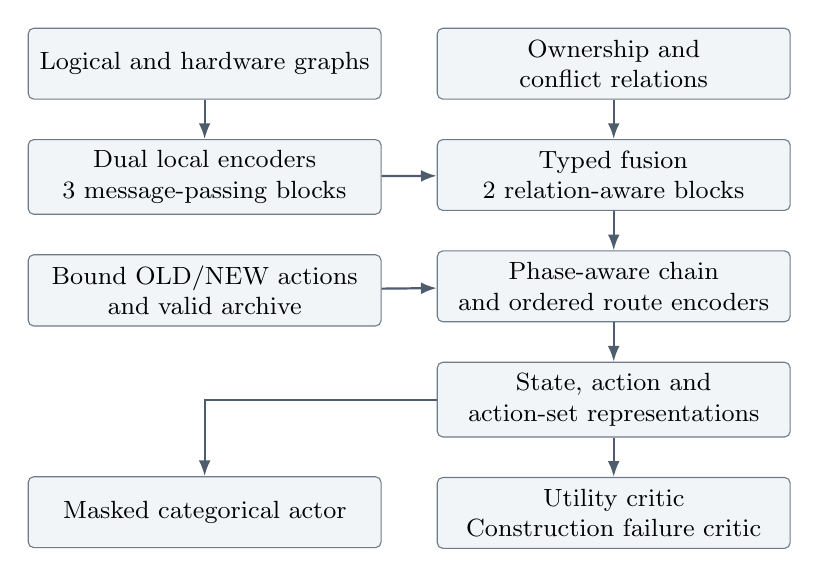
\begin{tikzpicture}[font=\small, node distance=5mm and 7mm,
 box/.style={draw=ink!65,rounded corners=2pt,fill=light,align=center,minimum height=9mm,text width=42mm,inner sep=4pt},
 arr/.style={-{Latex[length=2mm]},draw=ink!80,thick}]
\node[box] (g) {Logical and hardware graphs};
\node[box, right=of g] (o) {Ownership and conflict relations};
\node[box, below=of g] (e) {Dual local encoders\\3 message-passing blocks};
\node[box, below=of o] (f) {Typed fusion\\2 relation-aware blocks};
\node[box, below=of e] (p) {Bound OLD/NEW actions\\and valid archive};
\node[box, below=of f] (a) {Phase-aware chain\\and ordered route encoders};
\node[box, below=of a] (s) {State, action and\\action-set representations};
\node[box, below=of p, yshift=-14mm] (pi) {Masked categorical actor};
\node[box, below=of s] (v) {Utility critic\\Construction failure critic};
\draw[arr] (g)--(e); \draw[arr] (o)--(f); \draw[arr] (e)--(f);
\draw[arr] (f)--(a); \draw[arr] (p)--(a); \draw[arr] (a)--(s);
\draw[arr] (s)--(v); \draw[arr] (s.west)-|(pi.north);
\end{tikzpicture}
\caption{The trainable actor--critic. Exact candidate construction supplies full action payloads and a legal mask. A separate frozen strength predictor evaluates only valid terminal programs (Section 4.2).}
\end{figure}

\textbf{Implementation reading order:} Section 2 defines the RL task and
environment, Sections 3--4 define the networks, Sections 5.5--5.6 define
the complete loss and masks, Section 6 gives
collection/update/deployment algorithms, and Section 7.2 gives the
environment API and a numeric trajectory. Appendix A fixes every feature
slot. This revision completes the environment contract while retaining
the IF-Core-v1 network dimensions.

The model operates at \textbf{macro-decision epochs}. It selects a
complete, validated candidate rewrite rather than predicting individual
qubit memberships independently. The environment materializes
candidates, owns the masks, applies actions atomically, charges work and
validates final outputs. Learning changes action preferences and
continuation values. It never changes the definition of a valid
embedding.

The \textbf{actor and continuation critics} share trainable parameters
in a graph trunk. The \textbf{terminal strength selector} has
independent parameters and is frozen before PPO. Sharing weights across
the selector's four strength evaluations is allowed; sharing its
parameters with the PPO trunk is not part of IF-Core-v1.

\begingroup\small

\begin{longtable}[]{@{}
  >{\raggedright\arraybackslash}p{(\columnwidth - 6\tabcolsep) * \real{0.2200}}
  >{\raggedright\arraybackslash}p{(\columnwidth - 6\tabcolsep) * \real{0.4300}}
  >{\raggedright\arraybackslash}p{(\columnwidth - 6\tabcolsep) * \real{0.1500}}
  >{\raggedright\arraybackslash}p{(\columnwidth - 6\tabcolsep) * \real{0.2000}}@{}}
\toprule\noalign{}
\begin{minipage}[b]{\linewidth}\raggedright
Component
\end{minipage} & \begin{minipage}[b]{\linewidth}\raggedright
Function
\end{minipage} & \begin{minipage}[b]{\linewidth}\raggedright
Updated by PPO?
\end{minipage} & \begin{minipage}[b]{\linewidth}\raggedright
Needed for deployment?
\end{minipage} \\
\midrule\noalign{}
\endhead
\bottomrule\noalign{}
\endlastfoot
Exact environment and candidate generator & State transitions,
admissibility, budgets and final validation & No & Yes \\
Shared graph trunk & Current state and action representations & Yes &
Yes \\
Actor head & Distribution over the current legal macro-actions & Yes &
Yes \\
Utility critic & Expected raw terminal utility under the current policy
& Yes & No \\
Failure critic & Probability of no valid return in construction mode &
Construction only & No \\
Frozen strength selector & Predicted quality of a specified terminal
program at each strength & No & Yes \\
Independent evaluator & Fresh terminal training reward or assessment
counts & No & No, for embedding search \\
\end{longtable}

\endgroup

``Not needed for deployment'' means that critics and ground-truth
scoring are unnecessary for choosing an embedding. The returned physical
program is subsequently sampled by the actual solver as part of the
application workflow.

\hypertarget{rl-problem-and-environment-interface}{%
\section{RL problem and environment
interface}\label{rl-problem-and-environment-interface}}

\hypertarget{state-observation-and-operating-modes}{%
\subsection{State, observation and operating
modes}\label{state-observation-and-operating-modes}}

The logical Ising instance is \(I=(G_L,h,J)\), with energy

\[
E_I(s)=\sum_i h_i s_i+\sum_{(i,j)\in E_L}J_{ij}s_i s_j,
\qquad s\in\{-1,+1\}^{n}.
\tag{1}
\]

The active hardware graph is \(H\). The context \(\Omega\) fixes the
compiler, decoder, four chain strengths, sampler, feature schema,
candidate rules and budget units. Search state at a decision is

\[
s_t=(I,H,\Omega,\widetilde\phi_t,\mathcal O_t,\mathcal I_t,m_t,b_t,\mathcal K_t,M_t),
\qquad o_t=\operatorname{Tensorize}(s_t).
\tag{2}
\]

Here \(\widetilde\phi_t\) contains current branch sets;
\(\mathcal O_t(q)\) contains \textbf{all} logical claimants of hardware
vertex \(q\); \(\mathcal I_t\) is a valid-incumbent archive; \(m_t\)
holds current mode, ages, tabu and restart memory; \(b_t\) is the
remaining budget; and \(\mathcal K_t\) is the current candidate batch.
The state includes all transition-relevant search memory. The
finite-width neural representation is an approximation and is not
claimed to be injective or universally Markov sufficient.

Two modes have distinct initial-state and failure semantics:

\begin{itemize}
\tightlist
\item
  \textbf{Improvement mode, the first implementation:} initialize from a
  common valid embedding and retain it in a protected archive slot.
  Train the post-initialization policy on successful initializations.
  All ordinary completed episodes can return a valid incumbent.
  End-to-end accounting still includes initializer failures, which the
  subsequent actor cannot change.
\item
  \textbf{Construction mode:} initialize all chains empty and the
  archive empty. PLACE and ROUTE become available. Failure before an
  admissible incumbent exists is possible, so the failure critic and
  optional failure-constrained PPO are active.
\end{itemize}

Nonempty intermediate chains remain connected. Temporary overlap is
permitted only within the registered envelope. For occupancy
\(o(q)=|\mathcal O(q)|\), the initial envelope is

\[
\max_q o(q)\le2,\qquad
X=\sum_q(o(q)-1)_+\le\lceil0.1B_Q\rceil,
\qquad Q^{\rm unique}\le B_Q.
\tag{3}
\]

The environment also records \(Q^{\rm claim}=Q^{\rm unique}+X\). Final
outputs must be disjoint. Sharing a vertex does not realize a logical
edge: a valid contact requires a physical coupler between distinct
vertices in the two branch sets. The independent validator checks all
output conditions and faithful programming.

\hypertarget{complete-rl-specification-and-initial-state-distribution}{%
\subsection{Complete RL specification and initial-state
distribution}\label{complete-rl-specification-and-initial-state-distribution}}

The architecture is trained in a finite-horizon constrained Markov
decision process at macro-decision epochs:

\[
\mathfrak M_\Omega=(\mathcal S,\{\mathcal A(s)\}_{s\in\mathcal S},P_\Omega,
\mathcal R_\Omega,\mathcal C_\Omega,\rho_0,T_{\max},\gamma=1).
\tag{3a}
\]

\(P_\Omega\) is the environment transition kernel, not a learned
dynamics model. \(\mathcal R_\Omega\) and \(\mathcal C_\Omega\) give the
joint terminal reward/cost distribution; they are distinct from the
training reduction \(\mathcal R\) in Eq. (21). \(T_{\max}=32\) counts
\textbf{every selected macro-action, including COMMIT}. The task is
finite because each selected action consumes one decision and the other
work counters never increase.

Sample \((I,H)\) from the registered training distribution. For
improvement, the registered initializer, its seed distribution and
successful-initialization conditioning induce \(\rho_0\). The protected
initial embedding is independently checked before the first actor call.
For construction, set every chain empty, archive empty, all ages zero
and all budgets to their post-reset balances. A failed improvement
initializer is recorded as system initialization failure, without
inventing a post-initialization trajectory. The reference rollout
sampler uses unit episode weights; any alternative stratum weighting is
declared before collection.

The exact environment state includes the immutable input/context,
memberships, full ownership, archive, ages/tabu/restart memory, budget
counters and current candidate support. Reproducibility metadata
includes generator random state or independent substream counters.
Random draws are exogenous; the actor never receives a numeric random
seed as a feature. The initial distribution, transition rules and reward
event remain fixed during a training run. The compressed graph
representation may alias exact states; no claim of full observability
follows merely from choosing a GNN.

\hypertarget{four-different-meanings-of-validity}{%
\subsection{Four different meanings of
validity}\label{four-different-meanings-of-validity}}

Let \(C_i=\widetilde\phi(i)\) and let
\(H_{\rm act}=(V_{\rm act},E_{\rm act})\) be active hardware. Define the
number of unrealized logical demands by

\[
U(\widetilde\phi)=\sum_{(i,j)\in E_L}
\mathbf1\!\left\{\nexists\{q,r\}\in E_{\rm act}:q\in C_i,
\ r\in C_j,\ q\ne r\right\}.
\tag{3b}
\]

Membership overlap alone is never a contact. All logical-edge counts use
undirected edges once.

\textbf{Search-state admissibility, \(P_{\rm search}(x)\).} Every
logical ID has exactly one stored branch-set record, which may be empty
in construction. Improvement keeps every chain nonempty, including after
a restart. Every nonempty branch set lies in active hardware and is
connected in its active induced graph. Ownership equals the memberships
exactly, and all occupancy/conflict counters are recomputed
consistently. Unique qubit use and temporary overlap obey Eq. (3);
remaining binding budgets are nonnegative. Every archived entry passes
\(P_{\rm return}\) below under the same immutable context. Archive
protection, ages, tabu counters and restart counters obey their update
rules. Neither \(U=0\) nor pairwise disjointness is required for a live
search state. A corrupt ownership cache, disconnected nonempty chain,
inactive claimed vertex or negative budget is a contract violation, not
a low-reward state to train on.

\textbf{Complete graph embedding, \(P_{\rm embed}(\phi)\).} This
predicate is stronger:

\[
\begin{aligned}
P_{\rm embed}(\phi)={}&
\mathbf1\{\forall i:\varnothing\ne C_i\subseteq V_{\rm act},\ H_{\rm act}[C_i]\text{ connected}\}\\
&\cdot\mathbf1\{\forall i\ne j:\ C_i\cap C_j=\varnothing\}
\cdot\mathbf1\{U(\phi)=0\}
\cdot\mathbf1\{|\cup_iC_i|\le B_Q\}.
\end{aligned}
\tag{3c}
\]

This predicate applies to a branch assignment; it is not an
episode-terminal flag. Finding a valid embedding causes archive
admission and may be followed by further search.

\textbf{Return admissibility, \(P_{\rm return}(\phi;\Omega)\).} A
returned object must satisfy \(P_{\rm embed}\) and the registered
compiler/range/precision checks for all four strength programs needed by
the frozen selector. For each program, the actually programmed internal
edges must connect every chain. Logical fields and couplings must be
distributed faithfully on the chain-aligned subspace. In the exact
arithmetic contract, with positive global scale \(a_j\),

\[
\sum_{q\in C_i}\bar h_q^{(j)}=a_jh_i,
\qquad
\sum_{\substack{\{q,r\}\in E_{\rm act}\\q\in C_i,\ r\in C_k}}
\bar J_{qr}^{(j)}=a_jJ_{ik},\quad i\ne k.
\tag{3d}
\]

Absent logical couplings have \(J_{ik}=0\); no undeclared inter-chain
term may be introduced. Programmed internal ferromagnetic couplers
contribute a constant on aligned chains. Hardware limits and declared
coefficient-representation checks apply to the actual program bytes.
Floating-point compilation uses a fixed, unit-aware numerical
verification tolerance; coarse quantization cannot be called exact
faithfulness and requires an explicitly different compiler contract.
This validation does not prove that chains never break or that the
physical ground state decodes optimally. Those effects belong to
terminal solve quality.

\textbf{Legal action and terminal status.} \(M(s,a)\) specifies whether
a particular bound action may be applied now. The Boolean \(d\) states
whether the \textbf{transition} ends the episode. Neither is equal to
\(P_{\rm embed}\) or \(P_{\rm return}\) of the current workspace.

\begingroup\small

\begin{longtable}[]{@{}
  >{\raggedright\arraybackslash}p{(\columnwidth - 6\tabcolsep) * \real{0.3000}}
  >{\raggedright\arraybackslash}p{(\columnwidth - 6\tabcolsep) * \real{0.1300}}
  >{\raggedright\arraybackslash}p{(\columnwidth - 6\tabcolsep) * \real{0.2900}}
  >{\raggedright\arraybackslash}p{(\columnwidth - 6\tabcolsep) * \real{0.2800}}@{}}
\toprule\noalign{}
\begin{minipage}[b]{\linewidth}\raggedright
Situation
\end{minipage} & \begin{minipage}[b]{\linewidth}\raggedright
Search admissible?
\end{minipage} & \begin{minipage}[b]{\linewidth}\raggedright
Current embedding returnable?
\end{minipage} & \begin{minipage}[b]{\linewidth}\raggedright
Actor/critic training?
\end{minipage} \\
\midrule\noalign{}
\endhead
\bottomrule\noalign{}
\endlastfoot
Empty constructor with an available decision & Yes & No & Yes \\
Connected incomplete chains & Yes, within budgets/envelope & No & Yes \\
Connected chains with permitted overlap & Yes & No & Yes \\
Complete valid workspace, not yet committed & Yes & Yes after
programming checks & Yes; search may continue \\
Relaxed workspace with a protected valid archive & Yes & Workspace: no;
archive: yes & Yes; failure value is zero in protected improvement \\
Inactive membership, disconnected chain or corrupt ledger & No & No &
Abort/resume the integrity incident; do not fabricate a transition \\
Absorbing state after return or ordinary failure & Terminal & Already
resolved & No new actor row; its incoming terminal transition trains
normally \\
\end{longtable}

\endgroup

No learned validity classifier supplies any of these exact predicates.
No validity penalty is needed to replace the exact mask. The model may
learn that some admissible states have poor continuation value without
changing their admissibility.

\hypertarget{bound-actions-exact-preconditions-and-postconditions}{%
\subsection{Bound actions: exact preconditions and
postconditions}\label{bound-actions-exact-preconditions-and-postconditions}}

The opcode order is \texttt{PLACE}, \texttt{ROUTE},
\texttt{REWRITE\_ONE}, \texttt{REWRITE\_GROUP}, \texttt{REPAIR\_GROUP},
\texttt{RESTART}, \texttt{COMMIT}, \texttt{STOP}. There are at most 64
state-changing candidates, eight archive COMMIT candidates and a
possible STOP row; padded capacity is 73. A candidate is fully
materialized before scoring. Its record binds affected logical IDs, OLD
and NEW branch sets, route owners, memory effects, state fingerprint and
an application-work upper bound. Candidate identity is metadata, not a
learned scalar.

For a nonterminal state-changing candidate with affected set \(S_a\),
define the simultaneous membership replacement

\[
C_i^+=\begin{cases}C_{a,i}^{\rm new},&i\in S_a,\\ C_i,&i\notin S_a.\end{cases}
\qquad
\mathcal O^+(q)=\{i:q\in C_i^+\}.
\tag{3e}
\]

OLD memberships must match the decision state. Apply the entire
replacement before checking aggregate occupancy and contacts; do not
apply a group sequentially and reject an intermediate ordering artifact.
A nonempty chain cannot become empty in an ordinary rewrite. In the
registered improvement profile, two complete initializer outcomes are
generated, charged and authenticated before the first policy decision,
then held in an episode-local persistent cache. RESTART binds one unused
successful cache slot and consumes it atomically; it never invokes a
fresh initializer during proposal generation or policy execution. A
failed or already consumed slot supplies no action. Construction RESTART
binds the empty workspace, resets workspace-specific ages, and preserves
the archive; it is the explicit exception that can empty previously
placed chains. Both modes keep their mode and spent work. At most two
selected improvement restarts are available per episode; ordinary
proposals still consume their full metered work whether selected or
rejected.

\begingroup\small

\begin{longtable}[]{@{}
  >{\raggedright\arraybackslash}p{(\columnwidth - 4\tabcolsep) * \real{0.2300}}
  >{\raggedright\arraybackslash}p{(\columnwidth - 4\tabcolsep) * \real{0.3900}}
  >{\raggedright\arraybackslash}p{(\columnwidth - 4\tabcolsep) * \real{0.3800}}@{}}
\toprule\noalign{}
\begin{minipage}[b]{\linewidth}\raggedright
Opcode
\end{minipage} & \begin{minipage}[b]{\linewidth}\raggedright
Preconditions in addition to the common mask
\end{minipage} & \begin{minipage}[b]{\linewidth}\raggedright
Atomic postcondition
\end{minipage} \\
\midrule\noalign{}
\endhead
\bottomrule\noalign{}
\endlastfoot
PLACE & Construction mode; one currently empty logical chain; a bound
nonempty connected branch set & Install that branch set; existing
memberships outside the affected set stay fixed \\
ROUTE & Construction mode; selected unrealized logical demand with both
endpoint chains nonempty; all owner-consistent route segments are bound
& Replace affected endpoint chains with connected supersets that realize
the selected demand; all claimed path vertices have declared owners \\
REWRITE\_ONE & One currently nonempty chain; connected nonempty
replacement differs from OLD & Replace the chain; other contacts or
overlap may improve or worsen within the common envelope \\
REWRITE\_GROUP & Distinct nonempty affected chains; size 2, 3, 4 or 8;
at least one membership changes & Simultaneously install all
replacements; no monotone chain-length or solve-quality condition \\
REPAIR\_GROUP & Size 2, 3, 4 or 8; the group includes every claimant of
at least one selected conflict, or both endpoints of a selected
unrealized demand & Install connected replacements; target selection
distinguishes this opcode, but strict immediate defect reduction is not
required \\
RESTART & Remaining restart allowance; a mode-compatible complete
successor is already bound & Replace workspace; decrement
selected-restart allowance once; preserve the whole valid archive and
all spent work \\
COMMIT & Referenced archive entry exists and is admissible; a terminal
decision and terminal reserve fit & Independently revalidate that entry,
select strength and return it; terminal, regardless of current workspace
validity \\
STOP & Construction with empty archive and remaining decision allowance
& Return ordinary no-valid failure; terminal; never enabled alongside an
available valid archive \\
\end{longtable}

\endgroup

The shared legality rule for nonterminal candidates is

\[
\begin{aligned}
M(s,a)={}&\mathbf1\{\mathrm{Bound}(s,a)\}
\mathbf1\{\mathrm{Pre}_{\rm opcode}(s,a)\}\\
&\cdot\mathbf1\{P_{\rm search}(\mathrm{Apply}_{\rm dry}(s,a))=1\}\\
&\cdot\mathbf1\{\widehat w_{\rm app}(s,a)\preceq b_{\rm free}(s)\}.
\end{aligned}
\tag{3f}
\]

Here \(\mathrm{Bound}\) means a real, current candidate whose complete
payload matches the state; \(\preceq\) is coordinatewise budget
comparison. The dry successor includes known memory/counter changes;
archive admission requirements are included in the application budget
bound. A state-changing action also requires at least two decisions
remaining: its own and the reserved final decision. COMMIT/STOP use
their terminal-specific predicates instead of the nonterminal dry-state
rule. A predicted low probability of success never makes an otherwise
legal action illegal.

Identical complete successor, memory and charged-application semantics
are deduplicated; different provenance alone does not create duplicate
policy mass. Rejected proposals are charged but absent or masked. An
actor selecting a masked/stale action is an implementation error; it
does not trigger a learned self-loop penalty. Policy evaluation always
receives a nonempty legal support or an explicit terminal result.

\hypertarget{transition-kernel-prepare-decide-apply-prepare-once}{%
\subsection{Transition kernel: prepare, decide, apply, prepare
once}\label{transition-kernel-prepare-decide-apply-prepare-once}}

Separate the raw workspace \(x_t\) from the decision state \(s_t\). The
latter is \textbf{after} candidate generation and preparation charges.
One external preparation call produces either a live decision state or
an ordinary terminal event:

\[
\mathrm{Prepare}_\Omega(x_t,\xi_t)\longrightarrow
s_t=(x_t^{\rm charged},\mathcal K_t,M_t)
\quad\text{or}\quad \bot_{\rm fail}.
\tag{3g}
\]

Preparation uses interruptible proposal generation, materialization,
deduplication and dry admissibility checks. It charges rejected attempts
too. Static and phase-dependent feature work is metered. Reserve an
audited upper bound for current actor inference before exposing the
observation; record charged units and measured runtime separately.
Populate remaining-budget global channels only after those charges and
final mask construction. Cache the resulting observation and full
support. This ordering prevents a circular or stale budget feature while
ensuring inference is not free.

After the actor selects \(a_t\), \texttt{step} applies the already bound
candidate to the \textbf{charged} state. For a nonterminal operation, it
recomputes ownership/contacts, updates memories, independently validates
and admits the selected valid workspace, and prepares exactly one next
decision. Symbolically,

\[
P_\Omega(s'\mid s,a)=
\Pr_{\xi'}\{\mathrm{Prepare}_\Omega(\mathrm{Apply}_\Omega(s,a),\xi')=s'\}.
\tag{3h}
\]

Terminal COMMIT/STOP branches bypass next-state preparation. The
environment is deterministic conditional on all registered random draws;
the kernel accounts for fresh proposal/initializer randomness and
terminal evaluator randomness. It is not necessary to train a neural
transition predictor for this policy-gradient model.

The accounting identities are

\[
b_t^{\rm decision}=b_t^{\rm raw}-w_{\rm prep}(x_t),\qquad
b_{t+1}^{\rm raw}=b_t^{\rm decision}-w_{\rm app}(s_t,a_t).
\tag{3i}
\]

The decision coordinate of application work is one. Preparation costs
are sunk even if their proposals are not chosen. Materialization already
charged in preparation is not charged again as application work.
Admission validation, memory updates and actual application are separate
costs. No operation replenishes the total budget; RESTART only changes
workspace and its remaining restart allowance. An application exceeding
its audited bound is an integrity incident, not permission to make the
ledger negative.

\textbf{Archive timing.} Initialize the protected slot only from a
validated initializer. Subsequently, admit only the \textbf{selected,
realized} workspace after its independent return-admissibility check. A
hypothetical valid candidate never enters the archive merely because the
generator explored it. Preserve the protected slot in improvement; other
entries use deterministic FIFO eviction, including eight mutable slots
in construction. Deduplicate exact embedding/program context. On a
duplicate, retain its original age and FIFO position. New entries have
age zero. Membership changes cannot mutate archived records. Never store
evaluator outcomes in archive inputs.

\textbf{Memory timing.} Count ages in completed selected decisions, not
internal generator attempts. Increment surviving chain, claim,
occupancy, conflict, demand and archive ages once per nonterminal
action; reset an age when its defining membership/status changes or when
the item is newly created. Realized-demand age is zero;
unrealized-demand age counts since becoming unrealized. Removed items
lose their ages. A restart resets workspace ages to zero; surviving
archive ages still advance by one selected decision. For a new conflict
or claim use zero. Archive age does not reset on revisiting its
embedding. All choices are deterministic from the previous exact state
and selected successor.

The v1 default has tabu disabled: all tabu counters are known zero, and
no hidden tabu restriction changes proposals. A nonzero tabu variant
must version the tenure and opcode exemptions; it is not silently
activated by the presence of a tabu feature. A bound RESTART consumes a
restart token only if selected, although every proposed initializer
attempt consumes work. An unsuccessful initializer proposal adds no
RESTART action. Age/restart changes that distinguish successors are
included before deduplication and likelihood replay.

\hypertarget{termination-absorbing-states-and-reserve-semantics}{%
\subsection{Termination, absorbing states and reserve
semantics}\label{termination-absorbing-states-and-reserve-semantics}}

Use terminal reason codes \texttt{COMMIT}, \texttt{STOP\_NO\_VALID},
\texttt{BUDGET\_NO\_VALID} and \texttt{NO\_ACTION\_NO\_VALID}. Integrity
errors and missing evaluator results are external errors, not terminal
training labels. The terminal output records whether a valid embedding
was actually returned.

The reserve covers a final COMMIT decision, its bounded preparation and
actor inference, fresh independent validation, four program/selector
evaluations and one training reward-read block. It is available under
the same caps for every admitted archive entry. Search proposals may
spend only the free portion. At one decision remaining, or whenever
ordinary preparation cannot fit, skip state-changing generation: expose
COMMIT-only support if the archive is nonempty; otherwise emit ordinary
no-valid failure. The final decision is included in the cap of 32, not
an extra action outside the horizon.

In live construction with no archive, STOP is available if its costs
fit. In improvement after successful initialization, ordinary
termination always has a valid archive path. A state-changing action may
move from a returnable workspace to a permitted overlapping workspace
while preserving that path. In either mode, current validity by itself
never ends the episode and does not create a terminal reward.

A transition into \(\bot_{\rm return}\) pays \((r,c)=(K/N,0)\) once; a
transition into \(\bot_{\rm fail}\) pays \((0,1)\) once. Thereafter both
states are absorbing, with zero future rewards, zero future costs and
value zero:

\[
P(\bot\mid\bot)=1,\qquad r(\bot,\bot)=c(\bot,\bot)=0,
\qquad V_U(\bot)=V_f(\bot)=0.
\tag{3j}
\]

No actor is called in an absorbing state. The \textbf{incoming terminal
transition} is kept in PPO. If applying a nonterminal action followed by
next preparation exhausts the task without a valid archive, that same
transition gets \((r,c,d)=(0,1,1)\). Do not append a fictitious STOP
that was never selected. If construction reset resolves an ordinary
no-valid terminal before any decision, keep an episode record with
length zero and no transition row. A failed improvement initializer
instead returns \texttt{InitFailureRecord}: log its system outcome and
spent initialization work, and do not count it among the conditional PPO
episodes. Stop collection if the declared initialization-attempt cap is
reached before the required successful resets; do not fabricate the
missing episodes. A subsequent auto-reset observation belongs to a new
episode and is never used as the terminal bootstrap.

Task-budget exhaustion is \texttt{terminated=true}, with zero bootstrap.
An artificial collector cut of a still-live task is
\texttt{truncated=true} and would require next-state bootstrap; v1
disables these cuts by collecting complete episodes. An infrastructure
interruption resumes or aborts the affected rollout instead of assigning
a task-failure reward.

\begingroup\small

\begin{longtable}[]{@{}
  >{\raggedright\arraybackslash}p{(\columnwidth - 8\tabcolsep) * \real{0.3400}}
  >{\raggedright\arraybackslash}p{(\columnwidth - 8\tabcolsep) * \real{0.1200}}
  >{\raggedright\arraybackslash}p{(\columnwidth - 8\tabcolsep) * \real{0.1200}}
  >{\raggedright\arraybackslash}p{(\columnwidth - 8\tabcolsep) * \real{0.1400}}
  >{\raggedright\arraybackslash}p{(\columnwidth - 8\tabcolsep) * \real{0.2800}}@{}}
\toprule\noalign{}
\begin{minipage}[b]{\linewidth}\raggedright
Event returned by \texttt{step}
\end{minipage} & \begin{minipage}[b]{\linewidth}\raggedright
Reward \(r\)
\end{minipage} & \begin{minipage}[b]{\linewidth}\raggedright
Cost \(c\)
\end{minipage} & \begin{minipage}[b]{\linewidth}\raggedright
\texttt{terminated}
\end{minipage} & \begin{minipage}[b]{\linewidth}\raggedright
Next actor call
\end{minipage} \\
\midrule\noalign{}
\endhead
\bottomrule\noalign{}
\endlastfoot
Legal rewrite; next decision prepared & 0 & 0 & False & Yes, including
permitted overlap/incompleteness \\
Newly valid selected workspace admitted; search continues & 0 & 0 &
False & Yes \\
COMMIT with a valid return and fresh reward reads & \(K/N\) & 0 & True &
No \\
Voluntary STOP with empty archive & 0 & 1 & True & No \\
Post-action preparation cannot continue; archive empty & 0 & 1 & True &
No \\
Ordinary search budget ends; archive available & 0 & 0 & False & Yes, on
reserved COMMIT-only support \\
Invalid action, stale payload, corrupt state or missing reward reads &
No fabricated label & No fabricated label & External error &
Resume/abort under the integrity protocol \\
\end{longtable}

\endgroup

\hypertarget{deployable-terminal-objective}{%
\subsection{Deployable terminal
objective}\label{deployable-terminal-objective}}

For a valid embedding \(\phi\), the registered compiler creates four
programs \(\Pi_{\phi,F_j}\). A separate model \(q_\psi\) predicts a
probability for each program and selects

\[
j_\psi(\phi)=\arg\max_{j\in\{1,2,3,4\}}q_\psi(\Pi_{\phi,F_j}),
\qquad F_\psi(\phi)=F_{j_\psi(\phi)}.
\tag{4}
\]

Here \(a_{\phi,F_j}\), used below, denotes the compiler's global
positive rescaling factor, not a policy action. Ties use the lowest
strength index. The selector receives program and input features only.
It does not receive \(E_0\), a planted solution, a hidden embedding
witness or success counts. Its weights, normalization and calibration
are frozen before RL.

At training termination, an independent evaluator draws \(N_{\rm est}\)
fresh reads at the selected strength and computes

\[
\begin{aligned}
K_{\rm est}&=\sum_{r=1}^{N_{\rm est}}
\mathbf1\{E_I(D_\phi^{\rm MV}(z_r))\le E_0(I)+\varepsilon_I\},\\
R_T&=\begin{cases}K_{\rm est}/N_{\rm est},&A_T=1,\\0,&A_T=0,\end{cases}
\quad C_T=1-A_T.
\end{aligned}
\tag{5}
\]

\(A_T\) denotes a valid returned embedding. The trusted evaluator may
know the certified optimum; the deployed actor and selector do not.
Majority ties and the energy tolerance are fixed by \(\Omega\). The
initial floating-point tolerance is
\(\varepsilon_I=10^{-8}\max(1,\sum_i|h_i|+\sum_{ij}|J_{ij}|)\), with
exact comparisons preferred for exact coefficient representations. A
benchmark must ensure this tolerance does not merge distinct energy
levels.

For \(T\) selected actions indexed \(0,\ldots,T-1\), base rewards and
costs are zero except \(r_{T-1}=R_T\) and \(c_{T-1}=C_T\). Use
\(\gamma=1\). A valid zero-hit block is a legitimate reward zero.
Missing reads, compiler errors and integrity failures are not ordinary
unsuccessful samples and must not enter PPO as invented zero rewards.

Conditioned on the chosen terminal program and frozen selector, fresh
evaluation gives an unbiased sample mean of its registered success
probability. Solver-read correlation changes uncertainty estimation, not
the definition of the marginal mean. The actor's target is
\(J_U=\mathbb E[R_T]\), not the maximum of four noisy hit rates or a
cut/chain-length surrogate.

\hypertarget{typed-graph-representation}{%
\section{Typed graph representation}\label{typed-graph-representation}}

\hypertarget{input-projections-and-conventions}{%
\subsection{Input projections and
conventions}\label{input-projections-and-conventions}}

Appendix A defines all raw feature slots and incidence arrays. Eight
core object types contain a total of \textbf{120 named scalar slots},
represented as value/knownness pairs: 240 channels distributed across
types, plus an eight-way opcode. This is a schema count, not the input
dimension of a whole graph. Routes, chain factors and archive
descriptors have additional explicitly specified fields.

Set \(d=128\). Node/factor projectors are
\texttt{Linear(D,128)\ -\textgreater{}\ SiLU\ -\textgreater{}\ LayerNorm(128)}.
Edge/claim projectors use width 32. Continuous transformations are
deterministic and fitted on the training partition; missing values are
zero \textbf{after} transformation, with knownness zero. An observed
zero has knownness one. Nonnegative counts use \(\log(1+x)\); signed
count deltas use \(\operatorname{sgn}(x)\log(1+|x|)\).

All weights are trainable except the external strength selector. Use
separate parameters for logical and hardware streams and separate
parameters across layers. Directed graph storage contains both
orientations of each undirected edge. Active physical edges support
message passing; disabled nominal vertices/edges are retained as fault
observations where available but do not create active routing or
message-passing connectivity. Node padding is excluded from every pool.
Isolated real nodes remain in the graph.

The following conventions apply to every MLP unless explicitly
overridden: affine layers with bias, SiLU between hidden layers, linear
output, no dropout. LayerNorm follows only where stated. Empty mean/max
pools return zeros. Max pooling must exclude padding using an internal
sentinel and replace the result by zero only when the entire set is
empty.

\hypertarget{three-dual-local-blocks}{%
\subsection{Three dual local blocks}\label{three-dual-local-blocks}}

For stream \(r\in\{L,H\}\) and layer \(\ell\in\{0,1,2\}\), compute

\[
\begin{aligned}
m_{uv}^{r,\ell}&=\operatorname{MLP}^{r,\ell}_{288\to128\to128}
[z_u^\ell,z_v^\ell,e_{uv}],\\
a_v^{r,\ell}&=[\operatorname{mean}_{u\in\mathcal N_r(v)}m_{uv}^{r,\ell},
\operatorname{max}_{u\in\mathcal N_r(v)}m_{uv}^{r,\ell}],\\
z_v^{\ell+1}&=\operatorname{LN}\left(z_v^\ell+
\operatorname{MLP}^{r,\ell}_{384\to256\to128}[z_v^\ell,a_v^{r,\ell}]\right).
\end{aligned}
\tag{6}
\]

Messages concatenate two 128-dimensional nodes and one 32-dimensional
edge. Mean/max aggregation yields 256 channels. All updates within a
block read the previous block's node states; never overwrite nodes
sequentially during aggregation. Explicit degree features retain
cardinality information. The architecture follows the message-passing
framework of
\href{https://proceedings.mlr.press/v70/gilmer17a.html}{Gilmer et
al.~(2017)}. It is a typed message-passing model, not an undocumented
use of a generic ``GNN layer.''

\hypertarget{two-ownershipconflict-fusion-blocks}{%
\subsection{Two ownership/conflict fusion
blocks}\label{two-ownershipconflict-fusion-blocks}}

Create one conflict token \(X_q\) per contested qubit. The six
directional relation types are \(L\to H\), \(H\to L\) for all ownership
claims; \(L\to X\), \(X\to L\) for all claimants; and \(H\to X\),
\(X\to H\) for the contested qubit. Ownership relations use the
projected claim attributes. Other relations use a zero 32-dimensional
edge vector; relation-specific weights encode their type. Initialize
conflict tokens from their width-eight descriptors.

For each fusion block and each relation \(r\), use

\[
\begin{aligned}
m_{uv}^{r}&=\operatorname{MLP}^{r}_{288\to128\to128}[z_u,z_v,e_{uv}^{r}],\\
a_v^{r}&=[\operatorname{mean}m_{uv}^{r},\operatorname{max}m_{uv}^{r}],\\
u_v^r&=\mathbf1\{\deg_r(v)>0\}
\operatorname{MLP}^{r}_{384\to256\to128}[z_v,a_v^r],\\
z_v^+&=\operatorname{LN}\left(z_v+\sum_{r:\,\mathrm{dst}(r)=\mathrm{type}(v)}u_v^r\right).
\end{aligned}
\tag{7}
\]

The degree gate prevents biases from absent relations from creating
phantom messages. Use a node-type-specific output LayerNorm and
synchronous updates. Do not concatenate all relation aggregates into an
unspecified input width. A qubit claimed by three chains contributes all
three ownership incidences and all three claimant-to-conflict
incidences.

\hypertarget{phase-aware-edges-and-chain-factors}{%
\subsection{Phase-aware edges and chain
factors}\label{phase-aware-edges-and-chain-factors}}

For each affected chain \(i\) in action \(a\), create OLD and NEW
factors. For each archived chain create an ARCHIVE factor. Add a learned
128-dimensional role embedding from \texttt{\{OLD,\ NEW,\ ARCHIVE\}} to
its projected width-16 descriptor. This distinguishes an archive from an
old current chain even though both have \texttt{phase\_is\_new=0}.
Denote the resulting descriptor by \(d_{a,i}^{p}\).

Contextualize an undirected edge using endpoint features and its
projected raw attributes:

\[
\bar e_{uv}^{p}=\operatorname{MLP}_{288\to64\to32}
[z_u+z_v,|z_u-z_v|,e_{uv}^{p}].
\tag{8}
\]

The raw phase attributes must describe the \textbf{corresponding} old,
proposed or archived assignment. In particular, never copy the current
workspace's compiled coupling into a different archived program. When a
phase is nonprogrammable because of overlap, physical coefficient slots
are missing. Structural incidences remain available. Cache static terms
where safe; charge phase-dependent computation.

A physical contact realizing a logical edge must preserve the
physical-to-logical association. Define an edge-use embedding

\[
u_{\rm use}=\operatorname{MLP}_{66\to64\to32}
[\bar e_H^{p},\bar e_L^{p},\operatorname{onehot}_{\{\mathrm{CHAIN},\mathrm{LOGICAL}\}}].
\tag{9}
\]

For an internal chain edge, set \(\bar e_L^p=0\). Store which hardware
edge, logical edge and chain factor own each use. Pool only uses
incident to the factor in question.

A chain factor concatenates descriptor (128), owning logical node (128),
hardware-membership mean/max (256), edge-use mean/max (64), and
realized-logical-edge mean/max (64):

\[
b_{a,i}^{p}=\operatorname{MLP}_{640\to256\to128}
[d_{a,i}^{p},z_i,P_H(C_{a,i}^{p}),P_{\rm use}(a,i,p),P_L(a,i,p)].
\tag{10}
\]

Membership is an unordered set. All physical memberships, internal edges
and realized demands are retained as indexed relations. This encoder can
still compress distinct structures to similar vectors; it is not claimed
to be injective.

For action encoding, explicitly pair OLD and NEW factors by the key
\((a,i)\):

\[
b_{a,i}^{\Delta}=\operatorname{MLP}_{512\to256\to128}
[b_{a,i}^{\rm old},b_{a,i}^{\rm new},b_{a,i}^{\rm new}-b_{a,i}^{\rm old},z_i].
\tag{11}
\]

For PLACE, OLD is an explicitly empty branch set with valid empty-set
structural descriptors. Its factor is still encoded with the OLD role.
Do not pool all old and new chains separately and thereby discard which
old chain becomes which new chain. Archived chains use the same factor
encoder with the ARCHIVE role and do not require an old/new pair.

\hypertarget{ordered-route-encoding}{%
\subsection{Ordered route encoding}\label{ordered-route-encoding}}

A route stores a sequence of hardware vertices, an explicit logical
owner for each owned segment, the action reference and its phase. Split
a path into owner-consistent segments when ownership changes. For length
\(L\), the four positional fields are normalized position, start flag,
end flag and logical-attachment flag, paired with knownness to width
eight. For \(L=1\), normalized position is zero and both endpoint flags
are one.

Project positional features to 32, concatenate with the hardware
representation, and map \(160\to128\), then zero every padded position
immediately after this biased projection. Each of two route blocks is

\[
[u,v]=\operatorname{Conv1D}_{128\to256,k=3}(x),\qquad
x^+=\operatorname{Mask}\left(\operatorname{LN}[x+\tanh(u)\odot\sigma(v)]\right).
\tag{12}
\]

Use same padding, apply LayerNorm across channels, and zero padded
positions after \textbf{each} block. Pool real positions by mean, max,
first and last, then map \(512\to128\) to obtain \(r_0\). Bind the route
to its logical owner and phase with
\texttt{MLP(384-\textgreater{}128-\textgreater{}128)} on
\([r_0,z_i,t_p]\). The resulting route vector has width 128. No
positional encoding is applied to an unordered branch set.

\hypertarget{archive-and-action-representations}{%
\subsection{Archive and action
representations}\label{archive-and-action-representations}}

For archive entry \(k\), the five raw fields are age, protected flag,
admissible flag, qubit count and maximum chain length. Value/knownness
pairing gives width ten. With projected descriptor
\(d_k\in\mathbb R^{128}\),

\[
\iota_k=\operatorname{MLP}_{384\to256\to128}
[d_k,\operatorname{mean}_i b_{k,i}^{\rm archive},\operatorname{max}_i b_{k,i}^{\rm archive}],
\quad
\iota=\operatorname{MLP}_{256\to128}
[\operatorname{mean}_k\iota_k,\operatorname{max}_k\iota_k].
\tag{13}
\]

An empty archive has summary zero. Each entry's own membership and
program relations are encoded independently of current ownership. The
improvement archive uses one protected initial slot and seven
deduplicated FIFO slots. Construction has no protected initial slot and
uses up to eight deduplicated FIFO slots. Archive ordering is observed
through age; outcomes are not stored as policy inputs.

An action descriptor has 24 scalars with knownness plus the opcode,
width 56. Project it to 128 and concatenate joint-chain mean/max (256),
route mean/max (256), touched-conflict mean/max (256), and the
referenced archive token (128). The action encoder is
\texttt{MLP(1024-\textgreater{}256-\textgreater{}128)}, giving \(v_a\).
Nonreferencing actions use a zero archive token. COMMIT gathers its
actual archive token. RESTART binds its already materialized
initialization successor and work receipt before scoring.

Real admissible actions alone contribute to the action-set summary

\[
c_{\mathcal K}=\operatorname{MLP}_{256\to128}
[\operatorname{mean}_{a:M(a)=1}v_a,\operatorname{max}_{a:M(a)=1}v_a].
\tag{14}
\]

Pool current logical, hardware and conflict nodes by type-specific
mean/max: \(3\times256=768\) channels. Append archive summary 128 and
global context 64, then use
\texttt{MLP(960-\textgreater{}256-\textgreater{}128)} to obtain \(z_s\).
All pools are segmented by observation in a batch. A valid candidate in
one observation cannot influence another observation's denominator,
actor context or critic.

\hypertarget{actor-critics-and-terminal-strength-selector}{%
\section{Actor, critics and terminal strength
selector}\label{actor-critics-and-terminal-strength-selector}}

\hypertarget{masked-categorical-actor}{%
\subsection{Masked categorical actor}\label{masked-categorical-actor}}

The actor tower is
\texttt{MLP(512-\textgreater{}256-\textgreater{}128-\textgreater{}1)}:

\[
\ell_a=\operatorname{MLP}_\pi[v_a,z_s,c_{\mathcal K},v_a\odot z_s],
\qquad
\log\pi_\theta(a\mid o,\mathcal K,M)
=\ell_a-\operatorname{logsumexp}_{b:M(b)=1}\ell_b,
\tag{15}
\]

for legal \(a\); illegal entries are \(-\infty\). Sampling uses the
categorical distribution at temperature one. The legal-support policy
follows the invalid-action masking formulation studied by
\href{https://arxiv.org/abs/2006.14171}{Huang and Ontañón (2020)}. The
actor emits no parameterized chain set and no value used as a hard
validity mask. Moving candidate rows and all associated indices
consistently must simply permute actor probabilities.

The critic input is \([z_s,c_{\mathcal K}]\in\mathbb R^{256}\). Both
towers have dimensions
\texttt{256-\textgreater{}128-\textgreater{}64-\textgreater{}1}. Utility
output is linear. Failure output is a logit \(z_f\), transformed to
\(V_f=\sigma(z_f)\) in construction. Their meanings are

\[
V_U^\pi(o)=\mathbb E_\pi[R_T\mid o],\qquad
V_f^\pi(o)=\Pr_\pi(A_T=0\mid o),\qquad V_A=1-V_f.
\tag{16}
\]

These values average over the policy's future search and the remaining
budget. They are not the quality of a particular current embedding and
not optimal values \(V^*\). In protected-initializer improvement,
conditional failure is zero by the environment contract; report
\(V_f=0\), disable failure regression and omit the cost actor term. The
failure tower may be instantiated for API compatibility, but its
parameters are frozen in this mode. Whole-system initialization failure
is reported outside this conditional prediction.

\hypertarget{independent-frozen-strength-predictor}{%
\subsection{Independent, frozen strength
predictor}\label{independent-frozen-strength-predictor}}

The selector has its own three-local/two-ownership-fusion trunk, width
128, with no actions, route, conflict or archive modules. Its valid
input contains the logical graph, physical program and ownership at
\textbf{the evaluated strength \(F_j\)}. A single set of weights is
reused for all four strengths. This produces four outputs by four
conditioned evaluations, not four independent networks.

Pool logical and hardware mean/max vectors (512), append global context
(64), strength-index one-hot (4), and \(F_j,a_{\phi,F_j}\) (2). Use
\texttt{MLP(582-\textgreater{}128-\textgreater{}64-\textgreater{}1)}
with sigmoid. Physical coefficient channels and global scale slot 23
refer to this actual compiled program. Search-only fields are
consistently masked in both training and deployment; retain global slots
1--8, 13 and 15--23, recomputing all embedding-derived fields for the
evaluated embedding. For this head the qubit-cap value remains a
deployment context, not an outcome. The scalar pair follows the same
registered transformation policy as its corresponding global fields.
Mask search-age and tabu features in logical slots 17--18, hardware slot
16, logical-edge slot 6 and claim slot 1. The selector uses only the two
directional ownership relation types; conflict relation modules are
absent. All masks are identical during selector fitting and deployment.

Define

\[
S_I=\max\left(\epsilon_S,
\sqrt{\frac{\sum_i h_i^2+\sum_{ij}J_{ij}^2}{\max(1,n+|E_L|)}}\right),
\qquad (F_1,F_2,F_3,F_4)=(0.5,1,2,4)S_I
\tag{17}
\]

for the v1 registry. These ratios define the experiment and are frozen
before PPO; a different registry requires consistent recompilation and
labeling. The predictor must not replace actual terminal reward by its
prediction.

For count labels \((K_j,N_j)\), use stable normalized binomial
cross-entropy on the logit \(z_j\):

\[
\mathcal L_\psi=\frac{1}{4|\mathcal D_\psi|}
\sum_{\Pi\in\mathcal D_\psi}\sum_{j=1}^{4}
\left[-\frac{K_j}{N_j}\log\sigma(z_j)
-\left(1-\frac{K_j}{N_j}\right)\log(1-\sigma(z_j))\right].
\tag{18}
\]

Use \texttt{BCEWithLogits(z\_j,K\_j/N\_j)}. Every program--strength pair
has equal weight regardless of read count; this choice is explicit
rather than an accidental minibatch effect. Fit on training records and
a reserved training-side calibration partition. Then freeze parameters,
preprocessing and calibration before policy warm start and PPO. No PPO
gradient passes through \(q_\psi\).

\hypertarget{optimization-and-reinforcement-learning-procedure}{%
\section{Optimization and reinforcement-learning
procedure}\label{optimization-and-reinforcement-learning-procedure}}

\textbf{Where the losses are defined.} Eq. (18) trains the independent
strength predictor; Eq. (19) initializes action ranking; Eq. (20)
constructs actor advantages; Eq. (24) is the joint PPO training loss;
Eq. (25) updates the optional failure multiplier. Sections 5.5--5.6 are
the implementation reference for the loss. Rewards and state-validity
predicates are environment quantities, not additional unspecified neural
loss terms.

\hypertarget{supervised-initialization}{%
\subsection{Supervised initialization}\label{supervised-initialization}}

Optional supervised initialization uses complete state/action support
and a frozen continuation policy \(\mu\). A quality counterfactual
estimates \(Q^\mu(o,a)=\mathbb E[R_T\mid o,a,\mu]\), not \(Q^*(o,a)\). A
trajectory under that continuation can initialize the utility critic
with its terminal outcome. A candidate-specific \(Q^\mu\) label must not
be assigned directly to a state-only \(V_U\) target without the
action/continuation distribution that gives it meaning.

If \(B_o\) is a reliable tied best-action set inside an evaluated set
\(E_o\), use

\[
\mathcal L_{\rm rank}
=-\log\sum_{a\in B_o}
\frac{\exp\ell_a}{\sum_{b\in E_o}\exp\ell_b}.
\tag{19}
\]

If every legal action was evaluated, \(E_o\) is the full legal support.
If only a subset was evaluated, use this subset-normalized loss; do not
label every unevaluated action as inferior. The full support still
provides the model's input action context. Skip ranking rows whose
comparisons are unresolved instead of inventing precise winners. No
offline counterfactual row enters the PPO importance-ratio buffer.

For a clean first implementation, complete warm start before RL and set
all supervised auxiliary coefficients to zero during PPO. This separates
initialization from on-policy optimization. The frozen strength selector
is trained first because its identity defines the policy's reward
target.

\hypertarget{complete-episode-collection-and-behavior-snapshot}{%
\subsection{Complete-episode collection and behavior
snapshot}\label{complete-episode-collection-and-behavior-snapshot}}

Use \(M=64\) complete post-initialization episodes per rollout in
improvement, or 64 complete construction episodes. Copy a \textbf{frozen
behavior snapshot} of the shared trunk, actor and critics. Every
decision in this batch uses this same snapshot. No optimizer step occurs
until all episodes finish. Freeze generator rules, feature normalizers,
compiler/context and strength selector for the experiment.

The registered collector is
\texttt{synchronous-active-episode-waves-per-episode-pcg64-v1} under
schema \texttt{isingfold.ppo-collection-schedule}, version 1. Give every
episode an immutable global schedule index. Derive independent PCG64
streams from the training seed, update index, episode index and an
explicit \texttt{environment} or \texttt{policy} domain. Reset all
scheduled episodes, then batch one model forward over the current live
states in episode-index order; step each row once and repeat with the
surviving episodes. Therefore a peer's horizon, terminal state or
initializer retry count cannot move another episode's environment or
action-sampling stream. The exact schedule mapping is recorded in the
experiment contract and rollout replay metadata. Sequential
scalar-collector pilots and their checkpoints are incompatible with this
protocol and cannot be resumed as registered runs.

The collector calls \texttt{Env.reset} once per episode and
\texttt{Env.step} once per selected action. A returned DecisionState
already contains the charged support and semantic tensors; the collector
does not regenerate it. Compute old action probabilities and old critic
values, sample a legal action and retain the full input plus old
outputs. \texttt{Env.step} applies the bound action, updates
memories/archive and returns either the next prepared DecisionState or a
terminal record with reward/cost. Final reward reads are distinct from
selector fitting, warm start and previous adaptive PPO updates.

Do not store only detached node embeddings. PPO must recompute its
trainable graph trunk from semantic inputs for gradients to reach the
encoder. Candidate regeneration is also prohibited during PPO updates: a
fresh generator call can silently change the denominator and successor
represented by an action ID.

\hypertarget{gae-terminal-flags-and-critic-targets}{%
\subsection{GAE, terminal flags and critic
targets}\label{gae-terminal-flags-and-critic-targets}}

Let \(d_t=1\) for a \textbf{task terminal}, including COMMIT, ordinary
failure, or exhaustion of the task's registered budget. Terminal
bootstrap is zero. A collector fragment ending while a task is still
live is a \textbf{collector truncation} and requires the old next-state
value; it is not a failed episode. IF-Core-v1 collects complete episodes
and disables collector truncation. An infrastructure interruption aborts
or resumes the stored job; it is not fabricated into a reward.

Use generalized advantage estimation
(\href{https://arxiv.org/abs/1506.02438}{Schulman et al., 2016}). For
both utility and cost, compute once from detached old values:

\[
\begin{aligned}
\delta_t^U&=r_t+(1-d_t)V_{U,\rm old}(o_{t+1})-V_{U,\rm old}(o_t),\\
\delta_t^f&=c_t+(1-d_t)V_{f,\rm old}(o_{t+1})-V_{f,\rm old}(o_t),\\
\widehat A_t^j&=\delta_t^j+0.95(1-d_t)\widehat A_{t+1}^j,
\qquad j\in\{U,f\}.
\end{aligned}
\tag{20}
\]

Reset the recurrence between episodes. Before any epoch shuffle, form one
utility baseline over the full frozen rollout. Let
\(\mathcal I=\{(i,t):w_i>0,\ |\{a:M_{it}(a)=1\}|\ge2\}\) be the
positive-weight transitions at which the policy can choose between at
least two legal actions. The production actor transform is

\[
\bar A^U=\frac{\sum_{(i,t)\in\mathcal I}w_i\widehat A_{it}^U}
{\sum_{(i,t)\in\mathcal I}w_i},
\qquad
\widetilde A_{it}^U=\widehat A_{it}^U-\bar A^U.
\]

The same fixed episode/stratum weights used by Eq. (21) define the
center. Singleton-action rows do not set it because their policy gradient
is identically zero. Compute the center exactly once and store the
detached \(\widetilde A^U\) for every PPO epoch; never recenter an epoch
or minibatch. If \(\mathcal I\) is empty, or if the weighted RMS of
\(\widetilde A^U\) on \(\mathcal I\) is at most \(10^{-8}\), an
improvement-mode update is degenerate and must fail before an optimizer
step. Subtracting a scalar preserves the objective's units and contrast.
Do not divide by a standard deviation. Failure-cost advantages
\(\widehat A^f\) remain uncentered.

Use the raw terminal outcomes as Monte Carlo critic targets:
\(G_t^U=R_T\) and \(G_t^f=C_T\) for all states in the corresponding
complete episode. These are deliberately not
\(\widehat A^{\rm GAE}+V_{\rm old}\) and are not changed by actor
centering. The combination is a Monte Carlo critic with a GAE actor.
Per-minibatch whitening and separate cost/reward standardization are
disabled.

The registered transform identity is
\texttt{full-rollout-policy-controllable-weighted-mean-center-no-whitening-v1}.
It is part of rollout replay and run metadata. Pilot runs, rollout buffers
and checkpoints produced under the earlier raw-advantage rule are
algorithmically incompatible: do not resume, pool or compare them as
replications of this protocol. Restart every registered cell from its
frozen pre-PPO initialization.

Potential-based shaping is absent. In particular, adding
\(\Phi(o_{t+1})-\Phi(o_t)\) while imposing \(V'_U=V_U-\Phi\) cancels
exactly in each TD residual. It would not create a distinct GAE
algorithm. Sparse reward is handled here through initialization,
meaningful macro-actions and value learning.

\hypertarget{episode-sum-reduction-and-minibatch-weighting}{%
\subsection{Episode-sum reduction and minibatch
weighting}\label{episode-sum-reduction-and-minibatch-weighting}}

Let \(N_{\rm tr}=\sum_iT_i\), \(w_i\) be fixed stratum importance
weights (one under uniform sampling), and \(L_{\rm ref}=32\) a fixed
reference length. Define the actor reduction

\[
\mathcal R(f)=\frac{1}{ML_{\rm ref}}
\sum_{i=1}^{M}w_i\sum_{t=0}^{T_i-1}f_{it}.
\tag{21}
\]

The fixed scale does not change the desired episode-return optimum. Do
\textbf{not} divide each episode by its own length: an episode's policy
gradient is a sum over its decisions. For the reference run, sample
uniformly from the registered target episode distribution and set
\(w_i=1\). Optional importance weights are fixed density ratios between
target and sampling strata, normalized in expectation, never recomputed
from the observed batch. With a uniformly sampled transition minibatch
\(\mathcal B\), size \(B\), the unbiased batch estimator of this
reduction is

\[
\widehat{\mathcal R}_{\mathcal B}(f)
=\frac{N_{\rm tr}}{ML_{\rm ref}B}
\sum_{(i,t)\in\mathcal B}w_i f_{it}.
\tag{22}
\]

Apply the same reduction to the reward surrogate, cost surrogate and
entropy term. Use the actual \(B\) for a final short minibatch. Critic
regressions use an explicitly different, uniform-over-stored-states
mean. If graphs require memory-sized microbatches, accumulate properly
scaled loss sums for a 256-transition minibatch before one optimizer
step; graph size must not silently change the training weight.

\hypertarget{masked-ppo-losses}{%
\subsection{Masked PPO losses}\label{masked-ppo-losses}}

Recompute current probabilities on the \textbf{stored observation,
candidates and mask}. With detached old chosen-action log probability,

\[
\rho_t=\exp\{\log\pi_\theta(a_t\mid o_t,\mathcal K_t,M_t)
-\log\pi_{\rm old}(a_t\mid o_t,\mathcal K_t,M_t)\}.
\tag{23}
\]

The utility surrogate follows PPO
(\href{https://arxiv.org/abs/1707.06347}{Schulman et al., 2017}); the
cost envelope below is an explicitly specified engineering extension.
For PPO clip \(\epsilon=0.2\),

\[
\begin{aligned}
L_U&=\mathcal R\left[\min\{\rho_t\widetilde A_t^U,
\operatorname{clip}(\rho_t,0.8,1.2)\widetilde A_t^U\}\right],\\
L_f&=\mathcal R\left[\max\{\rho_t\widehat A_t^f,
\operatorname{clip}(\rho_t,0.8,1.2)\widehat A_t^f\}\right],\\
\mathcal L_{\rm PPO}&=-L_U+\lambda_fL_f-\beta_H\mathcal R[\mathcal H(\pi_\theta)]\\
&\quad+\tfrac12\operatorname{mean}[(V_U-G^U)^2]
+\tfrac12\operatorname{mean}\operatorname{BCEWithLogits}(z_f,G^f).
\end{aligned}
\tag{24}
\]

Omit both failure terms and use \(\lambda_f=0\) in improvement. In
construction, the maximum cost envelope preserves an adverse empirical
cost change; it is not a proven upper bound on the true policy failure
rate. Entropy is computed over legal actions only. Use stable
log-softmax/BCE implementations; do not exponentiate unbounded raw
logits manually.

One optimizer owns the shared trunk, actor and active critic parameters.
The shared trunk receives actor and critic gradients. Do not detach
critic inputs. Old log probabilities, old values, advantages, returns,
masks and \(\lambda_f\) are constants. A future split-trunk model must
declare separate parameter ownership; the same parameter must never be
stepped by two optimizers unintentionally.

The optional construction constraint is \(\mathbb E[C_T]\le d_f\), where
\(d_f\) is required when the failure constraint is enabled. With the
constraint disabled, keep \(\lambda_f=0\) while still fitting the
construction failure critic. Freeze \(\lambda_f\) during all four PPO
epochs. Then update once from the just-collected complete episode costs:

\[
\lambda_f^{k+1}=\max\left(0,\lambda_f^k+0.05
\left[\frac1M\sum_iw_iC_T^{(i)}-d_f\right]\right),
\qquad\lambda_f^0=0.
\tag{25}
\]

The step size 0.05 is a proposed engineering default. Thresholds are not
inferred from an individual minibatch or from test performance. Output
validity follows from the validator; constrained PPO does not guarantee
a valid-return-rate threshold at each iteration.

\hypertarget{loss-implementation-labels-and-masks}{%
\subsection{Loss implementation, labels and
masks}\label{loss-implementation-labels-and-masks}}

Equation (24) is the \textbf{loss minimized by backpropagation}. The
reward in Eq. (5) is an environment observation; the policy does not
directly backpropagate through solver samples, the exact transition or
the compiler. For protected improvement the active loss is

\[
\mathcal L_{\rm improve}=-L_U-\beta_H\mathcal R[\mathcal H(\pi_\theta)]
+\tfrac12\operatorname{mean}[(V_U-R_T)^2].
\tag{24a}
\]

For construction, add \(\lambda_fL_f\) when the failure constraint is
enabled, and always add the failure-critic BCE term from Eq. (24). The
failure head predicts eventual no-valid return, not whether the current
workspace is a complete embedding. Once a construction archive exists
and is protected by the same terminal reserve, ordinary eventual
no-valid failure is impossible; the still-active construction failure
head should learn target zero on these trajectories.

\begingroup\small

\begin{longtable}[]{@{}
  >{\raggedright\arraybackslash}p{(\columnwidth - 4\tabcolsep) * \real{0.2000}}
  >{\raggedright\arraybackslash}p{(\columnwidth - 4\tabcolsep) * \real{0.4900}}
  >{\raggedright\arraybackslash}p{(\columnwidth - 4\tabcolsep) * \real{0.3100}}@{}}
\toprule\noalign{}
\begin{minipage}[b]{\linewidth}\raggedright
Loss component
\end{minipage} & \begin{minipage}[b]{\linewidth}\raggedright
Exact target or reduction
\end{minipage} & \begin{minipage}[b]{\linewidth}\raggedright
Stage and gradient recipient
\end{minipage} \\
\midrule\noalign{}
\endhead
\bottomrule\noalign{}
\endlastfoot
Utility actor &
\(-\mathcal R[\min(\rho\widetilde A^U,\operatorname{clip}(\rho)\widetilde A^U)]\)
& PPO; actor and shared trunk \\
Failure-cost actor &
\(+\lambda_f\mathcal R[\max(\rho\widehat A^f,\operatorname{clip}(\rho)\widehat A^f)]\)
& Constrained construction; actor and shared trunk \\
Entropy & \(-\beta_H\mathcal R[-\sum_{a:M(a)=1}\pi(a)\log\pi(a)]\) &
PPO; actor and shared trunk \\
Utility critic & \(\tfrac12\operatorname{mean}[(V_U-R_T)^2]\) & PPO;
utility head and shared trunk \\
Failure critic &
\(\tfrac12\operatorname{mean}\operatorname{BCEWithLogits}(z_f,1-A_T)\) &
Construction; failure head and shared trunk \\
Tied-best-action warm start & Eq. (19), normalized only over evaluated
actions & Optional before PPO; actor and trunk \\
Strength predictor & Eq. (18), target \(K_j/N_j\) for each
program-strength pair & Separate pretraining; selector only, then
frozen \\
Failure multiplier & Eq. (25), projected ascent on episode failure minus
\(d_f\) & Manual scalar update after PPO epochs; no autograd \\
\end{longtable}

\endgroup

Do not add a binary ``current workspace valid'' target to \(V_f\). For
example, the protected improvement policy may deliberately enter an
overlapping workspace while retaining a valid archive; its conditional
no-valid-return label remains zero. A valid COMMIT with zero solver hits
has \((R_T,C_T)=(0,0)\), whereas an ordinary failed constructor has
\((0,1)\). The utility target alone cannot distinguish these outcomes;
the failure head is the component that distinguishes them in
construction.

The following masks are separate objects:

\begingroup\small

\begin{longtable}[]{@{}
  >{\raggedright\arraybackslash}p{(\columnwidth - 4\tabcolsep) * \real{0.2500}}
  >{\raggedright\arraybackslash}p{(\columnwidth - 4\tabcolsep) * \real{0.3400}}
  >{\raggedright\arraybackslash}p{(\columnwidth - 4\tabcolsep) * \real{0.4100}}@{}}
\toprule\noalign{}
\begin{minipage}[b]{\linewidth}\raggedright
Mask or flag
\end{minipage} & \begin{minipage}[b]{\linewidth}\raggedright
Applied to
\end{minipage} & \begin{minipage}[b]{\linewidth}\raggedright
Must not be used for
\end{minipage} \\
\midrule\noalign{}
\endhead
\bottomrule\noalign{}
\endlastfoot
Real-node/real-candidate padding mask & Segmented pooling and storage
padding & Declaring a hardware fault or a failure outcome \\
Exact legal-action mask \(M\) & Actor normalization, sampling, entropy
and categorical KL & Excluding an entire admissible observation from
training \\
Task-terminal flag \(d_t\) & Next-value bootstrap and GAE continuation &
Dropping the incoming terminal transition from actor/critic loss \\
Transition-row validity mask & Padded rollout rows only; all real
collected rows are true & Removing incomplete, overlapping or low-reward
search states \\
Current \(P_{\rm embed}\) / \(P_{\rm return}\) & Environment
admission/return logic and observable features & PPO loss masking or
instantaneous failure labels \\
Training mode / constraint flag & Activation of failure head and cost
actor term & Changing the recorded terminal event after observing its
outcome \\
\end{longtable}

\endgroup

A complete episode gives the training chain

\[
\text{terminal counts and return status}
\longrightarrow (R_T,C_T)
\longrightarrow (G^U,G^f,\widehat A^U,\widehat A^f)
\longrightarrow \mathcal L_{\rm PPO}
\longrightarrow \nabla_\Theta\mathcal L_{\rm PPO}.
\tag{24b}
\]

Counts, status, old outputs and computed targets are detached at this
boundary. The likelihood-ratio and current critic paths retain
gradients. GAE with \(\lambda_{\rm GAE}=0.95\) uses an approximate value
baseline and can introduce bias when that baseline is imperfect; the
minibatch reduction in Eq. (22) is unbiased for its stored full-buffer
surrogate, not a proof that the entire GAE/PPO update is an unbiased
exact policy gradient.

The following loss routine makes the reduction and numerical masks
explicit. \texttt{valid} indexes real transition rows in this minibatch,
and the actual size \(B\) is their count. All stored arrays have already
been detached; the forward pass recomputes the trainable network on the
saved semantic inputs.

\begin{verbatim}
new = model.forward(saved_observations, saved_candidates, saved_legal_mask)
logp_new = gather(new.masked_log_probs, chosen_actions)[valid]
rho = exp(logp_new - old_chosen_logp[valid])
rho_clip = clamp(rho, 0.8, 1.2)
su = minimum(rho * AU[valid], rho_clip * AU[valid])
sf = maximum(rho * Af[valid], rho_clip * Af[valid])  # construction only

# Never form 0 * (-infinity) for illegal entries.
logp_safe = where(legal_mask, new.masked_log_probs, 0)
p_legal = where(legal_mask, exp(new.masked_log_probs), 0)
entropy = -sum(p_legal * logp_safe, action_axis)[valid]

actor_reduce(f) = Ntr / (M * Lref * B) * sum(weight[valid] * f)
loss = -actor_reduce(su) - betaH * actor_reduce(entropy)
loss += 0.5 * mean(square(new.utility_value[valid] - GU[valid]))
if construction:
    loss += 0.5 * mean(BCEWithLogits(new.failure_logit[valid], Gf[valid]))
    if failure_constraint_enabled: loss += lambda_f * actor_reduce(sf)

optimizer.zero_grad()
loss.backward()                    # shared trunk and active heads
clip_global_grad_norm(parameters, 0.5)
optimizer.step()                   # one owner for each parameter
\end{verbatim}

The categorical ratio uses the chosen action, while entropy and KL use
the complete legal support. PPO has no replay across behavior-policy
batches and no target-Q network. The frozen old policy snapshot is its
behavior denominator, not an independently bootstrapped DQN target
network. The frozen strength model is a separate terminal control
module, not a substitute critic.

\hypertarget{probability-replay-kl-and-update-schedule}{%
\subsection{Probability replay, KL and update
schedule}\label{probability-replay-kl-and-update-schedule}}

Set all dropout probabilities in the PPO path to zero. Use LayerNorm
without running statistics, fixed input normalization and deterministic
graph encoding. No stochastic graph augmentation is applied between
rollout and likelihood replay. Evaluation mode and gradient recording
are separate: \texttt{model.eval()} can be used while autograd remains
enabled for PPO updates.

Before the first update, recomputed chosen-action log probabilities must
equal the saved values, within a registered float32 tolerance such as
\(10^{-5}\) in a controlled deterministic runtime. Thus
\(\rho_t\approx1\). A mismatch is a contract failure to investigate, not
a reason to widen PPO clipping.

Store full old categorical log probabilities to compute support-wise KL:

\[
\overline D_{\rm KL}
=\frac1{N_{\rm tr}}\sum_t\sum_{a:M_t(a)=1}
\pi_{\rm old}(a\mid o_t)
[\log\pi_{\rm old}(a\mid o_t)-\log\pi_\theta(a\mid o_t)].
\tag{26}
\]

This is a per-decision diagnostic mean, distinct from \(\mathcal R\).
Evaluate legal entries only to avoid \(0\cdot(-\infty-(-\infty))\).
Check KL after each epoch and stop subsequent epochs if the full-buffer
mean exceeds 0.02. A minibatch KL can be logged but must not be
mislabeled as the full-buffer value. This is an empirical early stop,
not a hard trust-region guarantee.

Use four shuffled epochs with the same stored targets. AdamW defaults
are learning rate \(3\times10^{-4}\), betas \((0.9,0.999)\), epsilon
\(10^{-5}\) and weight decay zero. Clip the combined gradient norm to
0.5. With declared total PPO update budget \(K_{\rm train}\), set
\(\beta_H(k)=0.01\max(0,1-k/(0.8K_{\rm train}))\). This schedule is
frozen before training. Do not add an unreported step penalty or time
discount.

\Needspace{47\baselineskip}

\hypertarget{algorithms-and-deployment}{%
\section{Algorithms and deployment}\label{algorithms-and-deployment}}

\Needspace{45\baselineskip}

\hypertarget{algorithm-1-complete-episode-masked-ppo}{%
\subsection{Algorithm 1: complete-episode masked
PPO}\label{algorithm-1-complete-episode-masked-ppo}}

\begin{verbatim}
Inputs: exact environment Env(Omega), frozen strength selector psi,
        initial PPO parameters Theta, M=64, E=4, B=256, Lref=32.
Set lambda_f=0. Declare mode and failure_constraint_enabled.
For update k = 0,...,Ktrain-1:
    Theta_old = detached copy of trunk, actor and active critics
    buffer = empty; every collection worker uses Theta_old
    assign M immutable global episode schedule indices
    For episode i = 1,...,M:
        derive independent environment and policy PCG64 streams for i
        repeat within the registered initialization-attempt cap:
            decision_or_terminal = Env.reset(instance, mode, environment_rng_i)
            if InitFailureRecord: log system failure/work; resample task
        until not InitFailureRecord  # failure to fill batch aborts collection
        episode_rows = empty
        if live: add (i, decision_or_terminal, policy_rng_i) to active
        else: store its resolved zero-transition terminal episode
    while active is nonempty:
        old_wave = batched_forward(Theta_old, active states in episode-index order)
        For each active (i, s, policy_rng_i) and matching old output:
            a = categorical_sample(old.masked_log_probs, policy_rng_i)
            result = Env.step(s, a)   # apply, then prepare next once
            save semantic s, full support, a, old outputs and result
            append transition index to episode_rows
            if result is live: retain its next state for the next wave
            else: store terminal reward/cost, weight and episode offsets
        # No fabricated transition when episode_rows is empty.
    if total transition count Ntr == 0: diagnose/stop collection
    verify unchanged-policy likelihood replay on the stored supports
    compute detached MC targets and raw GAE once, respecting episode offsets
    center utility GAE once over positive-weight policy-controllable rows
    reject a degenerate improvement signal; reuse centered values for all epochs
    freeze lambda_f for this PPO phase
    For epoch = 1,...,E:
        shuffle real transition indices with their ragged records
        For minibatch of at most B transitions:
            recompute current forward on saved semantic inputs
            minimize Eq. (24) using the loss routine in Section 5.6
        compute full-buffer legal-support KL, Eq. (26)
        if KL > 0.02: break
    if construction and failure_constraint_enabled:
        update lambda_f once using Eq. (25) and all M episode costs
    else: lambda_f=0
    log raw returns, costs, work and update diagnostics
    discard buffer; next collection uses the updated behavior snapshot
\end{verbatim}

\texttt{Env.step} resolves the independent terminal evaluator in
training mode: a valid COMMIT selects strength with the frozen selector,
obtains fresh counts, and emits \(R_T=K/N,C_T=0\); ordinary no-valid
failure emits \(R_T=0,C_T=1\). Intermediate outputs are zero reward and
cost. A preparation-induced terminal belongs to the selected action that
preceded it. Only the environment owns these labels. The learner never
rechecks workspace validity to overwrite them.

Ordinary environment failure is a valid training outcome.
Integrity/evaluator failure interrupts the affected job. Zero-decision
constructor episodes keep their terminal costs in the episode
denominator and dual estimate but contribute no actor/critic row. No
collection worker updates parameters before all 64 episodes in the
behavior batch are complete.

\Needspace{22\baselineskip}

\hypertarget{algorithm-2-inference-without-critics-or-ground-truth-labels}{%
\subsection{Algorithm 2: inference without critics or ground-truth
labels}\label{algorithm-2-inference-without-critics-or-ground-truth-labels}}

\begin{verbatim}
Load actor/trunk Theta, frozen selector psi, Omega and normalizers.
result = Env.reset(instance, mode, deployment_seed)
if result is InitFailureRecord: return initialization failure and work receipt
while result is a live DecisionState:
    s = result  # exact payloads and mask already prepared and charged
    logp = actor_forward(Theta, s.observation, s.candidates, s.legal_mask)
    a = categorical_sample(logp, temperature=1)
    step_result = Env.step(s, a, evaluate_training_reward=False)
    result = step_result.next_decision_or_terminal
if result is a valid TerminalRecord:
    return embedding, selected program/strength, validation/work receipts
else:
    return no-valid status and terminal reason
\end{verbatim}

The deployment \texttt{step} retains the same transitions, archive,
reserve, independent return validator and frozen strength choice. It
does not obtain a ground-truth reward block or know \(E_0\). It returns
the selected physical program for the application to sample.
Training-only reward/cost arrays are not model inputs. Critics may be
skipped. Greedy argmax or using a critic to perform beam search changes
the controller and must be named explicitly.

\hypertarget{implementation-contract}{%
\section{Implementation contract}\label{implementation-contract}}

\hypertarget{public-model-api}{%
\subsection{Public model API}\label{public-model-api}}

\begin{verbatim}
GraphActorCritic.forward(observation_batch, candidate_batch, legal_mask)
  -> {
       masked_log_probs: Float[Bobs,73],
       utility_value: Float[Bobs],
       failure_logit: Float[Bobs],   # active only in construction
       failure_value: Float[Bobs],  # exactly zero in protected improvement
       action_count: Int[Bobs]
     }

FrozenStrengthSelector.forward(valid_embedding_program_grid)
  -> success_logits: Float[Bembeddings,4]
\end{verbatim}

The selector API receives four fully compiled program contexts for each
embedding and evaluates the same network on each. The actor API accepts
variable-size graphs via concatenated tensors and graph-index arrays. A
single observation can have fewer than 73 candidates. Every
graph/factor/route node carries a batch ID or derives it from an owner
index. Relation endpoints must belong to the same observation. The
network never accepts a raw string digest as a differentiable feature.

For masked sampling, save the local candidate position and its stable
payload key. Positions support tensor gather; keys verify that the
gathered row still refers to the same successor. Return finite values on
real graphs, including empty conflict/archive sets. Do not rely on
implicit \texttt{nan\_to\_num} calls to repair undefined pooling or
all-false masks.

\Needspace{33\baselineskip}

\hypertarget{exact-environment-api-and-one-worked-trajectory}{%
\subsection{Exact environment API and one worked
trajectory}\label{exact-environment-api-and-one-worked-trajectory}}

\begin{verbatim}
Env.reset(instance, mode, seed)
  -> DecisionState | TerminalRecord | InitFailureRecord | EnvironmentError

DecisionState = {
    exact_state, observation, candidates, legal_mask,
    state_fingerprint, context_version, charged_work_receipt
}

Env.step(decision_state, chosen_local_index, evaluate_training_reward=True)
  -> StepResult | EnvironmentError

StepResult = {
    next_decision_or_terminal,
    reward, failure_cost, terminated, truncated=False,
    terminal_reason, work_receipt
}

TerminalRecord = {
    returned_valid, terminal_reason,
    embedding_or_none, selected_program_or_none, selected_strength_or_none,
    validation_receipt, cumulative_work,
    training_R_or_none, training_C_or_none, evaluator_counts_or_none
}
\end{verbatim}

\texttt{InitFailureRecord} contains an unsuccessful
improvement-initializer status and its work receipt, with no PPO
transition or conditional episode label. The initialization-attempt cap
is required collector configuration. \texttt{reset} prepares the first
support exactly once after an accepted initialization. \texttt{step}
checks the state fingerprint, current mask and chosen payload before
mutation; it prepares the next support exactly once when continuing. The
collected row is \((o_t,\mathcal K_t,M_t,a_t,r_t,c_t,d_t,o_{t+1})\) plus
frozen old outputs and replay metadata. A terminal next observation is
absent, never an auto-reset observation. In deployment the
training-label fields are absent. This API is an environment contract;
external compiler/sampler implementations remain configured
dependencies.

Consider an improvement trajectory beginning with a protected valid
seed. The first rewrite creates permitted overlap, the second repairs it
and creates another valid incumbent, and the third commits an archive
entry. Assume the independently observed terminal count is \(64/256\).

\begingroup\small

\begin{longtable}[]{@{}
  >{\raggedright\arraybackslash}p{(\columnwidth - 8\tabcolsep) * \real{0.2300}}
  >{\raggedright\arraybackslash}p{(\columnwidth - 8\tabcolsep) * \real{0.2100}}
  >{\raggedright\arraybackslash}p{(\columnwidth - 8\tabcolsep) * \real{0.2300}}
  >{\raggedright\arraybackslash}p{(\columnwidth - 8\tabcolsep) * \real{0.1700}}
  >{\raggedright\arraybackslash}p{(\columnwidth - 8\tabcolsep) * \real{0.1600}}@{}}
\toprule\noalign{}
\begin{minipage}[b]{\linewidth}\raggedright
\(t\) and selected action
\end{minipage} & \begin{minipage}[b]{\linewidth}\raggedright
Workspace before action
\end{minipage} & \begin{minipage}[b]{\linewidth}\raggedright
Workspace after action
\end{minipage} & \begin{minipage}[b]{\linewidth}\raggedright
\((r_t,c_t,d_t)\)
\end{minipage} & \begin{minipage}[b]{\linewidth}\raggedright
Old utility value
\end{minipage} \\
\midrule\noalign{}
\endhead
\bottomrule\noalign{}
\endlastfoot
0: REWRITE\_GROUP & Valid seed; archive nonempty & Connected permitted
overlap & \((0,0,0)\) & 0.10 \\
1: REPAIR\_GROUP & Permitted overlap & Valid, admitted to archive &
\((0,0,0)\) & 0.12 \\
2: COMMIT & Valid workspace; archive nonempty & Absorbing valid return &
\((0.25,0,1)\) & 0.18 \\
\end{longtable}

\endgroup

All three rows train. Row 1 is not removed because its input workspace
overlaps; row 2 is not removed because it is terminal. With old terminal
value zero, Eq. (20) yields

\[
\delta^U=(0.02,0.06,0.07),\qquad
\widehat A^U=(0.140175,0.1265,0.07),\qquad
G^U=(0.25,0.25,0.25).
\tag{27}
\]

Failure costs and improvement failure values are all zero; no failure
loss is active. Replacing the observed terminal count by zero would make
\(G^U=0\) while keeping \(C_T=0\). A different constructor trajectory
that never acquires an archive and stops has \(R_T=0,C_T=1\); every
earlier state in that episode gets failure MC target one. These are
eventual-return labels, not instantaneous geometry labels.

\hypertarget{rollout-buffer-schema}{%
\subsection{Rollout buffer schema}\label{rollout-buffer-schema}}

Let \(N_{\rm tr}=\sum_iT_i\) and \(M\) be the episode count.

\begingroup\small

\begin{longtable}[]{@{}
  >{\raggedright\arraybackslash}p{(\columnwidth - 4\tabcolsep) * \real{0.3000}}
  >{\raggedright\arraybackslash}p{(\columnwidth - 4\tabcolsep) * \real{0.2700}}
  >{\raggedright\arraybackslash}p{(\columnwidth - 4\tabcolsep) * \real{0.4300}}@{}}
\toprule\noalign{}
\begin{minipage}[b]{\linewidth}\raggedright
Field
\end{minipage} & \begin{minipage}[b]{\linewidth}\raggedright
Shape / type
\end{minipage} & \begin{minipage}[b]{\linewidth}\raggedright
Purpose
\end{minipage} \\
\midrule\noalign{}
\endhead
\bottomrule\noalign{}
\endlastfoot
Semantic observations and candidate payloads & Ragged records, length
\(N_{\rm tr}\) & Recompute the trainable trunk and exact support \\
Candidate padding mask; legal mask & Each \([N_{\rm tr},73]\), bool &
Distinguish absent rows from inadmissible real actions \\
Old masked log probabilities & \([N_{\rm tr},73]\), float32 & Exact
categorical KL on legal support \\
Chosen local action index & \([N_{\rm tr}]\), int64 & Gather likelihood
ratio \\
Chosen old log probability & \([N_{\rm tr}]\), float32 & Frozen behavior
denominator \\
Old utility and failure values & Each \([N_{\rm tr}]\), float32 &
Detached GAE inputs \\
Reward and cost & Each \([N_{\rm tr}]\), float32 & Nonzero only on
task-terminal transitions \\
Task-terminal; collector-truncated & Each \([N_{\rm tr}]\), bool & Zero
bootstrap versus live continuation \\
Episode index and offsets & \([N_{\rm tr}]\) and \([M+1]\), int64 &
Correct GAE resets and episode denominators \\
Terminal return, cost and stratum weight & Each \([M]\) & MC targets and
complete-episode dual update \\
Utility/cost GAE and MC targets & Four arrays \([N_{\rm tr}]\) &
Detached, reused for all PPO epochs \\
Context, generator, normalizer and selector versions & Metadata & Replay
and compatibility checks, not neural inputs \\
\end{longtable}

\endgroup

Masks, targets and old outputs do not require gradients. Store or
reconstruct next observations before any automatic reset. Collector
truncation is always false in the default complete-episode
implementation. Recurrent hidden state and replay-based off-policy
learning are absent.

\hypertarget{parameter-and-gradient-ownership}{%
\subsection{Parameter and gradient
ownership}\label{parameter-and-gradient-ownership}}

\begingroup\small

\begin{longtable}[]{@{}
  >{\raggedright\arraybackslash}p{(\columnwidth - 4\tabcolsep) * \real{0.3100}}
  >{\raggedright\arraybackslash}p{(\columnwidth - 4\tabcolsep) * \real{0.4100}}
  >{\raggedright\arraybackslash}p{(\columnwidth - 4\tabcolsep) * \real{0.2800}}@{}}
\toprule\noalign{}
\begin{minipage}[b]{\linewidth}\raggedright
Parameter group
\end{minipage} & \begin{minipage}[b]{\linewidth}\raggedright
Receives gradients from
\end{minipage} & \begin{minipage}[b]{\linewidth}\raggedright
Optimizer ownership
\end{minipage} \\
\midrule\noalign{}
\endhead
\bottomrule\noalign{}
\endlastfoot
Dual local encoders, fusion, factor/route/archive encoders & Actor loss
and active critic losses & One PPO optimizer \\
Actor tower & Reward surrogate, entropy, construction cost surrogate &
Same PPO optimizer \\
Utility tower & Utility MSE & Same PPO optimizer \\
Failure tower & Construction failure BCE & Same PPO optimizer; frozen in
improvement \\
Strength selector & Count loss before PPO only & Separate pretraining
optimizer, then frozen \\
Old policy snapshot & None & No optimizer \\
Masks, generators, decoder and compiler & None & Non-neural
environment \\
\end{longtable}

\endgroup

Avoid computing advantages from current critic outputs inside the actor
loss graph. Detach all advantage and target tensors once after
collection. Do not mix stale trajectories from earlier policies into
later PPO buffers without a separately defined off-policy method. If a
scalar configuration changes the action support, reward event or
selector, it changes the task registry rather than merely a model
checkpoint.

\hypertarget{reference-hyperparameters}{%
\subsection{Reference hyperparameters}\label{reference-hyperparameters}}

\begingroup\small

\begin{longtable}[]{@{}
  >{\raggedright\arraybackslash}p{(\columnwidth - 4\tabcolsep) * \real{0.2600}}
  >{\raggedright\arraybackslash}p{(\columnwidth - 4\tabcolsep) * \real{0.4300}}
  >{\raggedright\arraybackslash}p{(\columnwidth - 4\tabcolsep) * \real{0.3100}}@{}}
\toprule\noalign{}
\begin{minipage}[b]{\linewidth}\raggedright
Item
\end{minipage} & \begin{minipage}[b]{\linewidth}\raggedright
Registered value
\end{minipage} & \begin{minipage}[b]{\linewidth}\raggedright
Contract role
\end{minipage} \\
\midrule\noalign{}
\endhead
\bottomrule\noalign{}
\endlastfoot
Hidden width; local/fusion blocks & 128; 3 / 2 & IF-Core-v1 model
identity \\
Route blocks & 2 gated convolutions, kernel 3 & Fixed architecture \\
Candidate/commit capacity & 64 / 8; padded total 73 & Environment
contract \\
Archive & 1 protected + 7 FIFO & Profile-I environment value \\
Macro-decision cap & 32 & Profile-I value; includes and reserves
COMMIT \\
Selected restart allowance / tabu tenure & 2 / 0 & Profile-I value; no
hidden tabu mask \\
Rollout / minibatch & 64 complete episodes / 256 transitions & Main-grid
training value \\
PPO epochs / clip & 4 / 0.2 & Main-grid training value \\
Discount / GAE & 1 / 0.95 & Undiscounted objective / estimator
setting \\
Actor reference length & \(L_{\rm ref}=32\) & Frozen reduction
constant \\
AdamW & lr \(3\times10^{-4}\), betas \((0.9,0.999)\), eps \(10^{-5}\),
weight decay 0 & Main-grid optimizer value \\
Value loss weights & utility 0.5; construction failure 0.5 & Model-loss
contract \\
Dropout / stochastic tensor augmentation & 0 / disabled during PPO &
Likelihood-replay contract \\
Gradient norm / full-buffer KL stop & 0.5 / 0.02 & Registered
stabilizers \\
Entropy & 0.01 linearly to zero by \(0.8K_{\rm train}\) & Frozen
schedule \\
Failure dual & init 0; step 0.05; inactive in improvement & Construction
only \\
Terminal reward reads & 256 at selected strength & Training-side
sampling budget \\
Supervised loss during PPO & 0 & Clean warm-start-then-RL procedure \\
Deployment rule & Categorical sampling, temperature 1 & Same action
distribution as training \\
Training seeds & 1103, 2207, 3301 & All included in selection and
confirmation \\
\end{longtable}

\endgroup

\(K_{\rm train}\), compiler/evaluator settings and every native work cap
are required configuration fields. Construction additionally declares
\texttt{failure\_constraint\_enabled}; \(d_f\) is required when that
flag is true. There is no undocumented numerical default for a
scientific threshold. A terminal COMMIT is included in the 32-action
Profile-I cap; ordinary state-changing generation must leave room for it.

\hypertarget{complexity-and-implementation-checks}{%
\subsection{Complexity and implementation
checks}\label{complexity-and-implementation-checks}}

For fixed depth/width, sparse compute scales with logical/hardware
vertices and edges, current claims, conflict incidences, all OLD/NEW
route and edge-use incidences, and all archived memberships. A cap of 73
actions does not bound the size of their graph payloads. The route
convolution is linear in route length. Message MLPs introduce
width-dependent \(O(d^2)\) factors. No dense hardware attention is used.
Report parameter counts from the instantiated modules, not from an
unverified hand estimate.

Before running a large job, verify these contracts:

\begin{enumerate}
\def\labelenumi{\arabic{enumi}.}
\tightlist
\item
  Node/candidate permutations preserve values and permute probabilities;
  every segmented relation stays within its observation.
\item
  OLD, NEW and ARCHIVE use their own memberships and coefficients; joint
  replacements preserve chain identity.
\item
  Empty pools are finite; route padding is zero before and after
  convolutions; singleton action support has probability one and entropy
  zero.
\item
  Unchanged-policy replay gives ratios one; illegal support has zero
  probability; entropy/KL never multiply zero by an infinite log
  probability.
\item
  Preparation runs once at reset and once per continuing step. Only
  selected successors enter the archive; all work and terminal reserves
  remain charged.
\item
  GAE resets by episode; task terminals bootstrap zero; MC targets
  follow their own episode, including its incoming terminal transition.
\item
  Admissible overlapping/incomplete states participate in loss. Eventual
  failure labels never come from current workspace validity.
\item
  Unequal episode lengths and memory microbatches reproduce Eq. (21); no
  accidental per-episode length normalization appears.
\item
  Actor/critic gradients reach the shared trunk, never old outputs or
  the frozen selector. Verify clipping signs and finite zero/all-hit BCE
  targets.
\item
  Checkpoints restore parameters, optimizer, context, normalizers and
  random state; exhausted tasks never call all-false softmax or bypass
  the independent return validator.
\end{enumerate}

\hypertarget{scientific-artifact-and-selection-contract}{%
\subsection{Scientific artifact and selection
contract}\label{scientific-artifact-and-selection-contract}}

The model is only one component of the scientific system. Every
target-bearing process consumes a production prepared-v4 corpus plus a
publisher attestation whose record digest and publisher ID are pinned
out of band. Prepared v4 stores evaluator targets in physically
separate train, validation, and test files. Publisher attestation v2
binds the public prepared manifest, its partitioned target authority,
and separately hashed evidence manifests. The ground-certificate
protocol v2 publishes three target-bearing partition receipts and then
a target-free public root. Policy-facing planning authenticates only the
root. Selector fitting, label generation, training, and evaluation each
open only the partition required by that operation and retain the
resulting \texttt{TargetAccessReceipt} and ground-partition authority.

The artifact compatibility chain is fixed as follows: prepared schema
v4; selector-label manifest v4; selector bundle v4; quality rows v7;
quality shard and merge envelopes v5; quality preflight v2; release gate
v5; representation selection v4; RL-value freeze v4; scientific
checkpoint v3; and training-run receipt v4. Learned complete-system
receipts use v3 with evaluation report v4 and aggregate v2. External
tuning run and selection receipts use v2. External complete-system
receipts use v3 with report v4, and the paired learned-versus-stock
aggregate uses v4. Resumable evaluation uses plan v2, shard receipt v3,
and merge receipt v2. The final-strength diagnostic uses config v1,
sampler identity v1, plan v2, row v1, execution manifest v2, shard v1,
merge v1, and audit receipt v2. Re-signing an older artifact cannot
upgrade its semantics. A self-consistent digest without the externally
pinned publisher, ground-root, and selected-partition identities
establishes integrity, not authority, and is therefore insufficient.

The main architecture search is exactly (9+18) cells. The nine
representation cells cross IF-MLP, IF-Dual, and IF-Core with seeds 1103,
2207, and 3301. The eighteen RL-value cells cross the selected simpler
family and IF-Core with supervised-only, PPO warm-start, and
PPO-from-scratch training at the same three seeds. The test partition
remains sealed during both decisions. Family and method aggregates give
equal weight to every registered seed and immutable base lineage. Their
intervals use independent-with-replacement crossed resampling of the
seed and lineage axes, rather than treating the seed-by-lineage
observations as independent samples.

Before PPO collection, each training seed receives a sealed,
target-free deployment-initializer bank. Its plan assigns conditional
episodes equally over immutable train lineages and fixes a finite
sequence of LAC initializer draws for every episode. Generation stops at
the first successful draw, records all rejected draw work, and fails
closed if any episode exhausts its draw cap. Only after the bank and its
external manifest SHA-256 are authenticated may the training loader
attach the matching train-partition evaluator target. Thus PPO learns
the post-initializer Profile-I policy under an explicit conditional
distribution. Complete-system evaluation still begins before
initialization and scores every ordinary initializer failure as utility
zero.

After validation freezes one RL-value configuration, complete-system
confirmation freshly retrains all three registered seeds with no resume.
For supervised-only and PPO warm-start, the supervised representation is
also trained again from the authenticated quality-v7 corpus at that
seed. The counterfactual target remains
\texttt{if-q3-s0-qmu-5}. For PPO from scratch, model initialization is new. The selected
validation checkpoints identify the frozen configuration but are never
loaded into confirmation. A pre-existing confirmation destination is a
protocol error rather than an implicit resume.

Evaluation begins from the entire sealed policy-instance population
before initialization. Every failure has zero unconditional utility.
Detailed receipts partition failures into the pre-policy initializer
stage, policy-environment bootstrap, and post-bootstrap execution;
report summaries are recomputed from those receipts so an included
initializer failure cannot be mislabeled as an excluded row. Each valid
terminal return receives one independent 4096-read assessment at the
strength chosen by the frozen selector. The final aggregate
authenticates the three reports and all raw receipt, outcome, and
terminal-evidence sidecars before applying the registered crossed
bootstrap. Apollo and Goose may host different registered seeds, but
every configuration for a given seed must use the same runtime identity,
and validation repeats the training seed-to-host assignment.

Long learned, tuned-stock, and validation-tuning evaluations may be
resumed only through the common evaluation-shard protocol. A target-free
plan commits the complete public population, whole-lineage partition,
identity-derived seed schedule, run coordinates, and publication compute
class. A worker opens exactly the selected target partition, publishes
raw receipts, outcomes, terminal evidence, target-access authority, and
actual node provenance, then seals one shard receipt. Merge requires
every planned shard exactly once and recomputes the unsharded sufficient
statistics. Apollo publication workers use a pinned environment lock
directly. Goose workers run through Slurm and a pinned Apptainer runtime
and image. Bare-metal execution is diagnostic-only.

The registered LAC initializer v3 is prospectively bounded. Before each
call, the complete-system runner subtracts prior work and reserves the
invocation, candidate screen, environment bootstrap, and terminal policy
path. C++ checks each nine-coordinate delta before performing its
registered operation and returns a named
\texttt{WORK\_BUDGET\_EXHAUSTED} coordinate without crossing the cap.
Runtime identity includes SHA-256 digests of the loaded extension and
imported Python package sources, so a same-version binary replacement
cannot retain the same initializer identity.

Parameter capacity is not an axis in the main (9+18) selection. If
IF-Dual is the selected simpler family, the separately registered
diagnostic retrains width-128 IF-Core and a width-128,
nine-local-block IF-Dual control at all three paired seeds. The
trainable-parameter gap is bounded by 0.1 percent of the IF-Core
reference. This diagnostic cannot revise the main selection and cannot
establish pure architectural causality because depth and inference
compute still differ. It must report instantiated parameter counts,
latency, and peak accelerator memory.

Stock minorminer is tuned only on the full authenticated validation
population. A finite registry crosses the unmodified stock default with
time-saturating resource-ranked and frozen-selector quality-ranked
variants, each evaluated at all three registered seeds. One receipt
freezes the candidate, not a favorable seed, before test targets can be
opened. Test evaluation authenticates that selection and uses the same
pre-initialization population, pair keys, seed schedule, selector, final
evaluator, work caps, and total online wall-clock envelope as the
learned arm. The comparison does not claim equality between
solver-specific internal work coordinates.

The paired publication analysis uses a fixed-sequence familywise rule.
Valid-return noninferiority at margin 0.02 is tested first. Utility
superiority is confirmatory only when the noninferiority condition
passes, the paired unconditional IF-Q3-S0 lower confidence bound exceeds
zero, and the registered sample-size and precision guards pass.
Otherwise a positive point estimate does not establish superiority.

After model, stock candidate, and all three seeds are frozen, the
preregistered post-freeze diagnostic in
\texttt{configs/final\_strength\_audit\_v1.json} seals an outcome-blind,
stratum-balanced test subset. It requires at least 128 base lineages, no
more than 16 per signed stratum, 4,096 reads per block, 20,000 bootstrap
replicates, and exactly 128 shards. Its registry record digest is
\nolinkurl{fda50e04d2b193a26015f6f2c65c645e79bb9aaa05b346b9112505c06768c89e};
the registered file SHA-256 is
\nolinkurl{58497bdb40b2b83fb90208678f0644779753771045c9195df13d7697507e0c7c}.
All six source runs are authenticated and bound into a sealed execution
manifest before audit reads begin. For each valid return and each of the
four strengths, new block A reads choose the empirical oracle and
independent block B reads estimate
oracle-minus-deployed regret. Invalid returns remain in the coverage
denominator and receive a worst-case sensitivity range. Parallel
execution assigns complete opportunity keys to deterministic shards.
The merger requires the exact nonoverlapping shard census, authenticates
all rows and source evidence, restores canonical order, recomputes
summaries, and publishes atomically. Partial shards cannot enter a
claim. This audit is diagnostic and cannot modify training, either
selection receipt, or the primary endpoint. It is not primary evidence
for learned-method superiority.

\clearpage

\hypertarget{appendix-a.-tensor-and-feature-specification}{%
\section*{Appendix A. Tensor and feature
specification}\label{appendix-a.-tensor-and-feature-specification}}
\addcontentsline{toc}{section}{Appendix A. Tensor and feature
specification}

This appendix fixes the input contract of IF-Core. Scalar indices are
one-based within an object type. Indexing arrays carry identities and
relations; they are never concatenated as floating-point features. The
core schema has exactly \(20+18+6+10+6+4+24+32=120\) scalar slots,
\textbf{including} the 32 global slots. Knownness doubles these to 240
channels distributed across object types. Eight action-opcode indicators
are additional channels. Chain factors, route incidences, and archive
tokens are additional relational descriptors, whose widths are specified
separately.

\hypertarget{a.1-values-masks-units-and-program-contexts}{%
\subsection*{A.1 Values, masks, units, and program
contexts}\label{a.1-values-masks-units-and-program-contexts}}
\addcontentsline{toc}{subsection}{A.1 Values, masks, units, and program
contexts}

For \(D\) scalar slots, store
\(x=[\widetilde u_1,\ldots,\widetilde u_D,m_1,\ldots,m_D]\in\mathbb R^{2D}\).
Each \(m_j\) is one when the quantity is known and applicable. Unknown
values have \(\widetilde u_j=0,m_j=0\); observed zeros have \(m_j=1\).
Node padding, action padding, and action admissibility have separate
Boolean masks. A disabled hardware vertex is observed hardware, not
padding.

Apply fixed transforms before concatenating knownness. Coefficients and
coefficient-derived loads use
\(T_c(x)=\operatorname{sgn}(x)\log(1+|x|/c_{\rm train})\), with a
positive, recorded scale fitted using training inputs only and separate
scales for distinct physical units. Nonnegative counts, ages, distances,
and work use \(\log(1+x)\). Signed count or work differences use
\(\operatorname{sgn}(x)\log(1+|x|)\); in particular, action slots 6--10
and 18--19 must support negative values. Fractions, flags, and rescaling
factors remain bounded raw values. There is no per-instance coefficient
normalization that removes absolute energy scale. Deployment reuses the
same transforms and scales; missing values are zeroed after
transformation.

An empty combinatorial fraction is defined as known zero. A physically
undefined quantity is missing. Distances use active hardware support and
capped breadth-first search with a registry-fixed radius. A target
absent or unreachable within the cap is missing; a zero distance means
an actual intersection or identical endpoint. The exact record retains
the missingness reason. Counts use undirected edges once, even though
message-passing adjacency stores both orientations.

Compiled coefficients always identify a specific valid program context.
The current workspace uses reference strength \(F_1\). OLD, NEW, and
ARCHIVE program overlays use their own exact coefficients at \(F_1\), if
their complete applicable embedding has been compiled and validated.
Without that program, coefficient channels are missing. Current-program
coefficients must never be copied into an archived or candidate program
overlay. Static topology and calibration can be shared; phase-dependent
coefficient vectors cannot. For the terminal selector, overlay \(j\)
uses the actual \(F_j\) program and its rescaling factor. These overlays
reuse the schemas below and do not introduce new scalar types. Overlay
construction work is included in the environment ledger.

\hypertarget{a.2-logical-node-features-20-scalars-width-40}{%
\subsection*{A.2 Logical-node features: 20 scalars, width
40}\label{a.2-logical-node-features-20-scalars-width-40}}
\addcontentsline{toc}{subsection}{A.2 Logical-node features: 20 scalars,
width 40}

For logical node \(i\), write \(C_i\) for its current branch set and
\(\mathcal O(q)\) for all logical claimants of hardware vertex \(q\).

\begingroup\small

\begin{longtable}[]{@{}
  >{\raggedright\arraybackslash}p{(\columnwidth - 2\tabcolsep) * \real{0.1200}}
  >{\raggedright\arraybackslash}p{(\columnwidth - 2\tabcolsep) * \real{0.8800}}@{}}
\toprule\noalign{}
\begin{minipage}[b]{\linewidth}\raggedright
Slots
\end{minipage} & \begin{minipage}[b]{\linewidth}\raggedright
Exact scalar semantics
\end{minipage} \\
\midrule\noalign{}
\endhead
\bottomrule\noalign{}
\endlastfoot
1--4 & 1: signed field \(h_i\); 2: \(|h_i|\); 3: nonzero logical degree;
4: sum of incident \(|J_{ij}|\). \\
5--8 & 5: largest incident \(|J_{ij}|\); 6: signed incident coupling
sum; 7: positive-coupling fraction; 8: nonempty-chain flag. \\
9--12 & 9: \(|C_i|\); 10: programmed internal chain-edge count; 11:
induced active internal-edge count; 12: fraction of incident logical
demands with an active physical contact. \\
13--16 & 13: contested vertices claimed by \(i\); 14: maximum occupancy
on \(C_i\); 15: active boundary-edge count; 16: distinct active free
neighboring vertices outside \(C_i\). \\
17--20 & 17: decisions since this chain changed; 18: remaining tabu
decisions; 19: minimum active distance to an unrealized neighboring
chain; 20: nonempty connectedness flag. \\
\end{longtable}

\endgroup

Boundary edges have exactly one endpoint in \(C_i\). Realized contact
requires an active edge between the two branch sets, not merely a shared
vertex. Contact availability in a relaxed workspace does not imply
physical programmability. Programmed-edge count is missing without an
applicable program; induced-edge count remains structural. An empty
chain has connectedness zero. If no unrealized neighbor exists, slot 19
is missing rather than an artificial distance zero.

\hypertarget{a.3-hardware-node-features-18-scalars-width-36}{%
\subsection*{A.3 Hardware-node features: 18 scalars, width
36}\label{a.3-hardware-node-features-18-scalars-width-36}}
\addcontentsline{toc}{subsection}{A.3 Hardware-node features: 18
scalars, width 36}

\begingroup\small

\begin{longtable}[]{@{}
  >{\raggedright\arraybackslash}p{(\columnwidth - 2\tabcolsep) * \real{0.1200}}
  >{\raggedright\arraybackslash}p{(\columnwidth - 2\tabcolsep) * \real{0.8800}}@{}}
\toprule\noalign{}
\begin{minipage}[b]{\linewidth}\raggedright
Slots
\end{minipage} & \begin{minipage}[b]{\linewidth}\raggedright
Exact scalar semantics
\end{minipage} \\
\midrule\noalign{}
\endhead
\bottomrule\noalign{}
\endlastfoot
1--4 & 1: active flag; 2: active degree; 3: nominal degree; 4: occupancy
\(|\mathcal O(q)|\). \\
5--8 & 5: occupancy exceeds one; 6: active-neighbor free fraction; 7:
active-neighbor occupied fraction; 8: faulty-neighbor fraction among
nominal neighbors. \\
9--12 & 9: distinct claimants on active neighboring vertices; 10: signed
compiled bias; 11: compiled-bias magnitude; 12: maximum incident
compiled-coupling magnitude. \\
13--16 & 13: measured bias offset; 14: measured bias-noise standard
deviation; 15: readout error rate; 16: decisions since occupancy last
changed. \\
17--18 & 17: active distance to the nearest free vertex; 18: distinct
active vertices reachable in at most two hops, excluding \(q\). \\
\end{longtable}

\endgroup

An active free vertex has slot 17 equal to known zero. Disabled vertices
have missing active-distance values. If only active hardware support is
available, nominal degree and fault-neighborhood fractions are missing.
Calibration inputs come from the declared hardware snapshot. Unused
programmable vertices have known zero programmed bias when a full valid
program exists.

\hypertarget{a.4-logical-and-hardware-edges}{%
\subsection*{A.4 Logical and hardware
edges}\label{a.4-logical-and-hardware-edges}}
\addcontentsline{toc}{subsection}{A.4 Logical and hardware edges}

Logical edge \((i,j)\) has six scalars, width 12.

\begingroup\small

\begin{longtable}[]{@{}
  >{\raggedright\arraybackslash}p{(\columnwidth - 2\tabcolsep) * \real{0.1200}}
  >{\raggedright\arraybackslash}p{(\columnwidth - 2\tabcolsep) * \real{0.8800}}@{}}
\toprule\noalign{}
\begin{minipage}[b]{\linewidth}\raggedright
Slot
\end{minipage} & \begin{minipage}[b]{\linewidth}\raggedright
Semantics
\end{minipage} \\
\midrule\noalign{}
\endhead
\bottomrule\noalign{}
\endlastfoot
1--3 & 1: signed \(J_{ij}\); 2: \(|J_{ij}|\); 3: active-contact realized
flag. \\
4--6 & 4: number of active physical inter-chain edges; 5: shortest
active distance between branch sets; 6: decisions since this demand
became unrealized. \\
\end{longtable}

\endgroup

Age is known zero while the demand is realized. Distance is missing if
either branch set is empty or the capped search finds no path. Hardware
edge \((q,r)\) has ten scalars, width 20.

\begingroup\small

\begin{longtable}[]{@{}
  >{\raggedright\arraybackslash}p{(\columnwidth - 2\tabcolsep) * \real{0.1200}}
  >{\raggedright\arraybackslash}p{(\columnwidth - 2\tabcolsep) * \real{0.8800}}@{}}
\toprule\noalign{}
\begin{minipage}[b]{\linewidth}\raggedright
Slots
\end{minipage} & \begin{minipage}[b]{\linewidth}\raggedright
Exact scalar semantics
\end{minipage} \\
\midrule\noalign{}
\endhead
\bottomrule\noalign{}
\endlastfoot
1--3 & 1: active flag; 2: shared-claimant count
\(|\mathcal O(q)\cap\mathcal O(r)|\); 3: number of distinct unordered
logical pairs with one claimant at each endpoint, excluding
self-pairs. \\
4--7 & 4: programmed chain-edge flag; 5: programmed logical-coupler
flag; 6: signed compiled coupling; 7: compiled-coupling magnitude. \\
8--10 & 8: measured coupling offset; 9: measured coupling-noise standard
deviation; 10: fraction of endpoint claim incidences located at
contested endpoints. \\
\end{longtable}

\endgroup

The denominator of slot 10 is \(|\mathcal O(q)|+|\mathcal O(r)|\).
Program flags are missing for an invalid workspace. A valid unused
coupler has known zero flags and coefficient. A nominal disabled edge
remains observable, while routing and contact counts use active edges
only.

\hypertarget{a.5-claims-and-conflicts}{%
\subsection*{A.5 Claims and conflicts}\label{a.5-claims-and-conflicts}}
\addcontentsline{toc}{subsection}{A.5 Claims and conflicts}

Each claim \((i,q)\) contributes six scalars, width 12. A vertex claimed
by three chains produces three separate incidences.

\begingroup\small

\begin{longtable}[]{@{}
  >{\raggedright\arraybackslash}p{(\columnwidth - 2\tabcolsep) * \real{0.1200}}
  >{\raggedright\arraybackslash}p{(\columnwidth - 2\tabcolsep) * \real{0.8800}}@{}}
\toprule\noalign{}
\begin{minipage}[b]{\linewidth}\raggedright
Slots
\end{minipage} & \begin{minipage}[b]{\linewidth}\raggedright
Exact scalar semantics
\end{minipage} \\
\midrule\noalign{}
\endhead
\bottomrule\noalign{}
\endlastfoot
1--3 & 1: decisions since this claim was created; 2: contested flag; 3:
active neighbors of \(q\) inside \(C_i\). \\
4--6 & 4: active chain-boundary vertex flag; 5: articulation flag in the
active induced chain graph; 6: distinct realized incident logical
demands with a physical contact attached at \(q\). \\
\end{longtable}

\endgroup

Articulation uses the graph-theoretic component-increase definition;
singleton chains have flag zero. Each contested vertex \(q\)
additionally creates conflict factor \(X_q\), with four scalars, width
8: \textbf{1} excess occupancy \(|\mathcal O(q)|-1\); \textbf{2}
decisions since this vertex became contested; \textbf{3} distinct
claimants on active neighboring vertices; \textbf{4} adjacent active
free-vertex count. It connects to \(q\) and every claimant, irrespective
of insertion order.

\hypertarget{a.6-global-context-32-scalars-width-64}{%
\subsection*{A.6 Global context: 32 scalars, width
64}\label{a.6-global-context-32-scalars-width-64}}
\addcontentsline{toc}{subsection}{A.6 Global context: 32 scalars, width
64}

\begingroup\small

\begin{longtable}[]{@{}
  >{\raggedright\arraybackslash}p{(\columnwidth - 2\tabcolsep) * \real{0.1200}}
  >{\raggedright\arraybackslash}p{(\columnwidth - 2\tabcolsep) * \real{0.8800}}@{}}
\toprule\noalign{}
\begin{minipage}[b]{\linewidth}\raggedright
Slots
\end{minipage} & \begin{minipage}[b]{\linewidth}\raggedright
Exact scalar semantics
\end{minipage} \\
\midrule\noalign{}
\endhead
\bottomrule\noalign{}
\endlastfoot
1--4 & 1: logical vertices; 2: nonzero logical edges; 3: active hardware
vertices; 4: active hardware edges. \\
5--8 & 5: unique-qubit cap \(B_Q\); 6: currently claimed union size; 7:
total excess occupancy; 8: total unrealized logical demands. \\
9--12 & 9: remaining decision fraction; 10: remaining aggregate
deterministic-work fraction; 11: remaining restart count; 12: archive
entry count. \\
13--16 & 13: workspace-valid flag; 14: protected-seed-available flag;
15: absolute instance RMS coefficient scale \(S_I\); 16: maximum
magnitude among logical fields and couplings. \\
17--20 & 17: \(F_1\); 18: \(F_2\); 19: \(F_3\); 20: \(F_4\), all
expressed in pre-scale coefficient units. \\
21--24 & 21: symmetric hardware field limit; 22: symmetric hardware
coupler limit; 23: applicable program rescaling factor; 24:
improvement-mode flag. \\
25--28 & Remaining fractions for 25: route expansions; 26: candidate
materializations; 27: compiler calls; 28: validator calls. \\
29--32 & Remaining fractions for 29: cut-edge visits; 30:
initialization/restart work; 31: reserved terminal work; 32:
feature/inference work. \\
\end{longtable}

\endgroup

Every fraction uses its own registered cap. IF-Core fixes these caps, or
fixes a deterministic cap function of exposed instance sizes, so
fractions reconstruct absolute availability. Nonbinding coordinates are
missing; an exhausted binding coordinate is known zero. The Profile-I
decision cap is 32 and route-expansion cap is 200,000. All remaining cap
values and units must be instantiated in the immutable registry before
collection; unsupported coordinates cannot silently become free work.
Different hidden cap profiles are unsupported. Asymmetric signed
hardware limits require a versioned context extension, not compression
into these two symmetric-limit slots.

For the terminal selector, search-only slots 9--12, 14, and 24--32 are
missing. Embedding-derived slots are recomputed for the selected valid
embedding, and slot 23 uses its actual \(F_j\) program. The four v1
strengths are \((0.5,1,2,4)S_I\). Also mask logical-node slots 17--18,
hardware-node slot 16, logical-edge slot 6 and claim slot 1 in the
selector; these are search ages or tabu memory. Valid-program
coefficients and structural features are recomputed, not inherited from
a different workspace.

\hypertarget{a.7-bound-action-descriptors-24-scalars-plus-opcode-width-56}{%
\subsection*{A.7 Bound-action descriptors: 24 scalars plus opcode, width
56}\label{a.7-bound-action-descriptors-24-scalars-plus-opcode-width-56}}
\addcontentsline{toc}{subsection}{A.7 Bound-action descriptors: 24
scalars plus opcode, width 56}

\begingroup\small

\begin{longtable}[]{@{}
  >{\raggedright\arraybackslash}p{(\columnwidth - 2\tabcolsep) * \real{0.1200}}
  >{\raggedright\arraybackslash}p{(\columnwidth - 2\tabcolsep) * \real{0.8800}}@{}}
\toprule\noalign{}
\begin{minipage}[b]{\linewidth}\raggedright
Slots
\end{minipage} & \begin{minipage}[b]{\linewidth}\raggedright
Exact scalar semantics
\end{minipage} \\
\midrule\noalign{}
\endhead
\bottomrule\noalign{}
\endlastfoot
1--5 & 1: affected chains; 2: old claim incidences; 3: new claim
incidences; 4: added claims; 5: removed claims. \\
6--10 & Successor-minus-current differences in 6: claimed union size; 7:
maximum chain length; 8: total excess occupancy; 9: contested vertices;
10: unrealized demands. \\
11--15 & 11: resulting maximum occupancy; 12: resulting
structural-validity flag; 13: resulting qubit-cap slack; 14: charged
proposal work; 15: bound application-work upper bound. \\
16--20 & 16: maximum route length; 17: mean route length; 18:
affected-boundary-edge difference; 19: affected-free-neighbor
difference; 20: remaining restarts after application. \\
21--24 & 21: referenced archive age; 22: referenced archive union size;
23: restores an archived structure; 24: changes workspace. \\
\end{longtable}

\endgroup

Affected-boundary and free-neighbor differences sum the corresponding
per-chain quantities over the affected logical IDs. These may count one
physical item for multiple chains by design. Work descriptors use the
registered aggregate work unit; exact vector costs remain in the record
and drive masking. Every difference uses the same affected set in
predecessor and successor. COMMIT/STOP-inapplicable fields are missing.
Append the one-hot order
\texttt{PLACE,\ ROUTE,\ REWRITE\_ONE,\ REWRITE\_GROUP,\ REPAIR\_GROUP,\ RESTART,\ COMMIT,\ STOP}.
A batch contains at most 64 state-changing actions, eight COMMIT
actions, and one STOP row. Padding does not create a valid action.

\hypertarget{a.8-additional-factors-and-relational-indices}{%
\subsection*{A.8 Additional factors and relational
indices}\label{a.8-additional-factors-and-relational-indices}}
\addcontentsline{toc}{subsection}{A.8 Additional factors and relational
indices}

Each OLD, NEW, or ARCHIVE chain factor has eight scalars, width 16:
\textbf{1} phase-is-new; \textbf{2} branch-set size; \textbf{3} induced
active-edge count; \textbf{4} programmed chain-edge count; \textbf{5}
boundary-edge count; \textbf{6} contested claimed-vertex count in that
phase; \textbf{7} nonempty connectedness; \textbf{8} membership changed
from OLD. ARCHIVE factors set slots 1 and 8 to known zero. A learned
128-dimensional role embedding from \texttt{\{OLD,\ NEW,\ ARCHIVE\}} is
added to the projected descriptor, preserving the 640-dimensional factor
input. Pair OLD and NEW factors by \((a,i)\), not by row order.

A route incidence has four values plus knownness, width 8: normalized
position, start flag, end flag, logical-attachment flag. Position is
\(k/\max(L-1,1)\) for zero-based \(k\); a singleton has both endpoint
flags one. Routes retain order and claimant identity. Unordered branch
sets have no positional features.

An archive entry has exactly five scalars, width 10: \textbf{1} age;
\textbf{2} protected flag; \textbf{3} independently admissible flag;
\textbf{4} qubit use; \textbf{5} maximum chain length. Its chain factors
carry complete archived memberships and program-edge references. Archive
age counts decisions. Archive identity is an index, never a trainable ID
embedding.

\begingroup\small

\begin{longtable}[]{@{}
  >{\raggedright\arraybackslash}p{(\columnwidth - 2\tabcolsep) * \real{0.3000}}
  >{\raggedright\arraybackslash}p{(\columnwidth - 2\tabcolsep) * \real{0.7000}}@{}}
\toprule\noalign{}
\begin{minipage}[b]{\linewidth}\raggedright
Tensor or relation
\end{minipage} & \begin{minipage}[b]{\linewidth}\raggedright
Shape and interpretation
\end{minipage} \\
\midrule\noalign{}
\endhead
\bottomrule\noalign{}
\endlastfoot
\(X_L,X_H,X_{E_L},X_{E_H}\) & \((n,40),(m,36),(e_L,12),(e_H,20)\); edge
counts are directed. \\
\(I_L,I_H\) & \((2,e_L),(2,e_H)\) endpoint indices; both directions for
undirected edges. \\
\(I_O,X_O\) & \((2,M),(M,12)\); all logical-to-hardware claims. \\
\(X_X,I_{XL},I_{XH}\) & \((n_X,8),(2,M_X),(2,n_X)\);
conflict-to-claimant and conflict-to-host links, plus reverse
relations. \\
\(X_g,X_A\) & \((b,64),(A,56)\); disjoint-batch globals and candidate
descriptors. \\
\(X_B,I_{BA},I_{BL},I_{BH}\) & \((B,16)\); factor-to-action,
logical-owner, and membership indices each shaped
\((2,N_{\rm relation})\). Archive factors instead link to entry IDs. \\
Edge-use records & Each row stores chain-factor ID, physical-edge ID,
logical-edge ID when applicable, and role \texttt{\{CHAIN,\ LOGICAL\}};
absent logical-edge IDs are guarded before gather. \\
Route records & Route-to-action, route-to-logical-owner, phase, ordered
hardware IDs, and \((P_R,8)\) positional-incidence features. \\
\(X_Z,I_{BZ},I_{AZ}\) & \((Z,10)\) archive descriptors; factor-to-entry
and COMMIT-to-entry relations. \\
Batch and masks & Node/action/factor batch IDs; Boolean real-row masks
and exact candidate-admissibility masks; at most eight archive entries
per observation. \\
\end{longtable}

\endgroup

Features enter as float32, indices as int64, and masks as Boolean. Every
relation endpoint is offset independently when batching disjoint graphs.
Pooling is segmented by observation, action, factor, or archive entry as
appropriate; no incidence may cross observations. Store canonical
semantic records and exact candidate supports for likelihood replay.
Ground energies, planted assignments, evaluator counts, generator
provenance, and identifier hashes are excluded from learned channels.

\hypertarget{references}{%
\section*{References}\label{references}}
\addcontentsline{toc}{section}{References}

Gilmer, J., Schoenholz, S. S., Riley, P. F., Vinyals, O., and Dahl, G.
E. (2017).
\href{https://proceedings.mlr.press/v70/gilmer17a.html}{Neural Message
Passing for Quantum Chemistry}. \emph{Proceedings of the 34th
International Conference on Machine Learning}, PMLR 70:1263--1272.

Schulman, J., Moritz, P., Levine, S., Jordan, M., and Abbeel, P. (2016).
\href{https://arxiv.org/abs/1506.02438}{High-Dimensional Continuous
Control Using Generalized Advantage Estimation}. \emph{International
Conference on Learning Representations}.

Schulman, J., Wolski, F., Dhariwal, P., Radford, A., and Klimov, O.
(2017). \href{https://arxiv.org/abs/1707.06347}{Proximal Policy
Optimization Algorithms}. arXiv:1707.06347.

Huang, S. and Ontañón, S. (2020).
\href{https://arxiv.org/abs/2006.14171}{A Closer Look at Invalid Action
Masking in Policy Gradient Algorithms}. arXiv:2006.14171.

\emph{Project provenance:} \texttt{ISINGFOLD\_RL\_ARCHITECTURE\_EN.tex},
revised architecture produced in this project session; original
\texttt{PROJECT\_HANDBOOK\_EN.tex}, model diagrams and their
accompanying source manifest. This document makes explicit choices where
the previous model description left aggregation, masking, gradient flow
or probability reduction unspecified.

\textbf{Build:} Compile twice with
\texttt{pdflatex\ ISINGFOLD\_MODEL\_SPEC.tex}. The TeX source embeds its
figure and references. Markdown and PDF specify the same model and
algorithms.
\end{document}
